%%%%%%%%%%%%%%%%%%%%%%%%%%%%%%%%%%%%%%%%%
% Tufte-Style Book (Minimal Template)
% LaTeX Template
% Version 1.0 (5/1/13)
%
% This template has been downloaded from:
% http://www.LaTeXTemplates.com
%
% License:
% CC BY-NC-SA 3.0 (http://creativecommons.org/licenses/by-nc-sa/3.0/)
%
% IMPORTANT NOTE:
% In addition to running BibTeX to compile the reference list from the .bib
% file, you will need to run MakeIndex to compile the index at the end of the
% document.
%
%%%%%%%%%%%%%%%%%%%%%%%%%%%%%%%%%%%%%%%%%

%----------------------------------------------------------------------------------------
%	PACKAGES AND OTHER DOCUMENT CONFIGURATIONS
%----------------------------------------------------------------------------------------

\documentclass{tufte-book} % Use the tufte-book class which in turn uses the tufte-common class

\hypersetup{colorlinks} % Comment this line if you don't wish to have colored links

\usepackage{microtype} % Improves character and word spacing

\usepackage{lipsum} % Inserts dummy text

\usepackage{booktabs} % Better horizontal rules in tables

\usepackage{tikz}

\usepackage{menukeys}

\usepackage{enumitem}
	
\usepackage{amssymb}

\usepackage[utf8]{inputenc}

\usepackage{graphicx} % Needed to insert images into the document
\graphicspath{{Images/}} % Sets the default location of pictures
\setkeys{Gin}{width=\linewidth,totalheight=\textheight,keepaspectratio} % Improves figure scaling

\usepackage{fancyvrb} % Allows customization of verbatim environments
\fvset{fontsize=\normalsize} % The font size of all verbatim text can be changed here

\newcommand{\hangp}[1]{\makebox[0pt][r]{(}#1\makebox[0pt][l]{)}} % New command to create parentheses around text in tables which take up no horizontal space - this improves column spacing
\newcommand{\hangstar}{\makebox[0pt][l]{*}} % New command to create asterisks in tables which take up no horizontal space - this improves column spacing

\usepackage{xspace} % Used for printing a trailing space better than using a tilde (~) using the \xspace command

\newcommand{\monthyear}{\ifcase\month\or January\or February\or March\or April\or May\or June\or July\or August\or September\or October\or November\or December\fi\space\number\year} % A command to print the current month and year

\newcommand{\openepigraph}[2]{ % This block sets up a command for printing an epigraph with 2 arguments - the quote and the author
\begin{fullwidth}
\sffamily\large
\begin{doublespace}
\noindent\allcaps{#1}\\ % The quote
\noindent\allcaps{#2} % The author
\end{doublespace}
\end{fullwidth}
}

\newcommand{\blankpage}{\newpage\hbox{}\thispagestyle{empty}\newpage} % Command to insert a blank page

\usepackage{makeidx} % Used to generate the index
\makeindex % Generate the index which is printed at the end of the document



%----------------------------------------------------------------------------------------
%	BOOK META-INFORMATION
%----------------------------------------------------------------------------------------

\title{On Autodesk Revit} % Title of the book

\author{Bern Staples} % Author

\publisher{Northlake Christian School} % Publisher

%----------------------------------------------------------------------------------------

\begin{document}

%----------------------------------------------------------------------------------------

\maketitle % Print the title page

%----------------------------------------------------------------------------------------
%	COPYRIGHT PAGE
%----------------------------------------------------------------------------------------

\newpage
\begin{fullwidth}
~\vfill
\thispagestyle{empty}
\setlength{\parindent}{0pt}
\setlength{\parskip}{\baselineskip}
Copyright \copyright\ \the\year\ \thanklessauthor

\par\smallcaps{Published by \thanklesspublisher}

\par\smallcaps{http://www.northlakechristian.org}

\par\smallcaps{Special thanks to Thomas Morton}

\par  This information is free; you can redistribute it and/or modify it
    under the terms of the GNU General Public License as published by
    the Free Software Foundation; either version 2 of the License, or
    (at your option) any later version.

    This work is distributed in the hope that it will be useful,
    but WITHOUT ANY WARRANTY; without even the implied warranty of
    MERCHANTABILITY or FITNESS FOR A PARTICULAR PURPOSE.  See the
    GNU General Public License for more details.
    
    The source code of this document may be found under a public GIT repository here: \url{http://www.github.com/hendenburg/onautodeskrevit}

    You should have received a copy of the GNU General Public License
    along with this work; if not, write to the Free Software
    Foundation, Inc., 51 Franklin Street, Fifth Floor, Boston, MA 02110-1301, USA.\index{license}
    
    \newthought{This document utilizes} the Tufte-Style Book formating method. It utilizes formating and functions of this template. The Template may be found at \url{http://www.LaTeXTemplates.com} and the template is under an individual CC BY-NC-SA 3.0 license.  
\par\textit{First printing, \monthyear}
\end{fullwidth}

%----------------------------------------------------------------------------------------

\tableofcontents % Print the table of contents

%----------------------------------------------------------------------------------------

\listoffigures % Print a list of figures

%----------------------------------------------------------------------------------------




%----------------------------------------------------------------------------------------
%	INTRODUCTION
%----------------------------------------------------------------------------------------

\cleardoublepage
\chapter{Introduction} % The asterisk leaves out this chapter from the table of contents
\label{ch:0}

The following guide and user manual utilizes Autodesk Revit, a BMI program which is used to create Architectural Visualizations \cite{revit2016}. The guide is based on Autodesk's own guide \cite{guide2006}

%------------------------------------------------

\section{Starting Revit}


To start Revit, either find the program via its icon, or by searching for \menu{Revit} by bringing up the search menu with the \keys{Windows Key}

\section{Getting adjusted to Revit}
The Figure \ref{fig:revmainscene} represents an accurate representation of a Revit opening screen. When opening a Revit project file this screen is circumvented.

\section{Starting your first project, and an introduction to Revit's interface}
Let's antiquate ourselves with the introduction page. The introduction page is made up of two primary sections: \menu{Projects} and \menu{Families}. For the time being you can ignore the \menu{Families} section, and focus only on the former.

\begin{figure}
	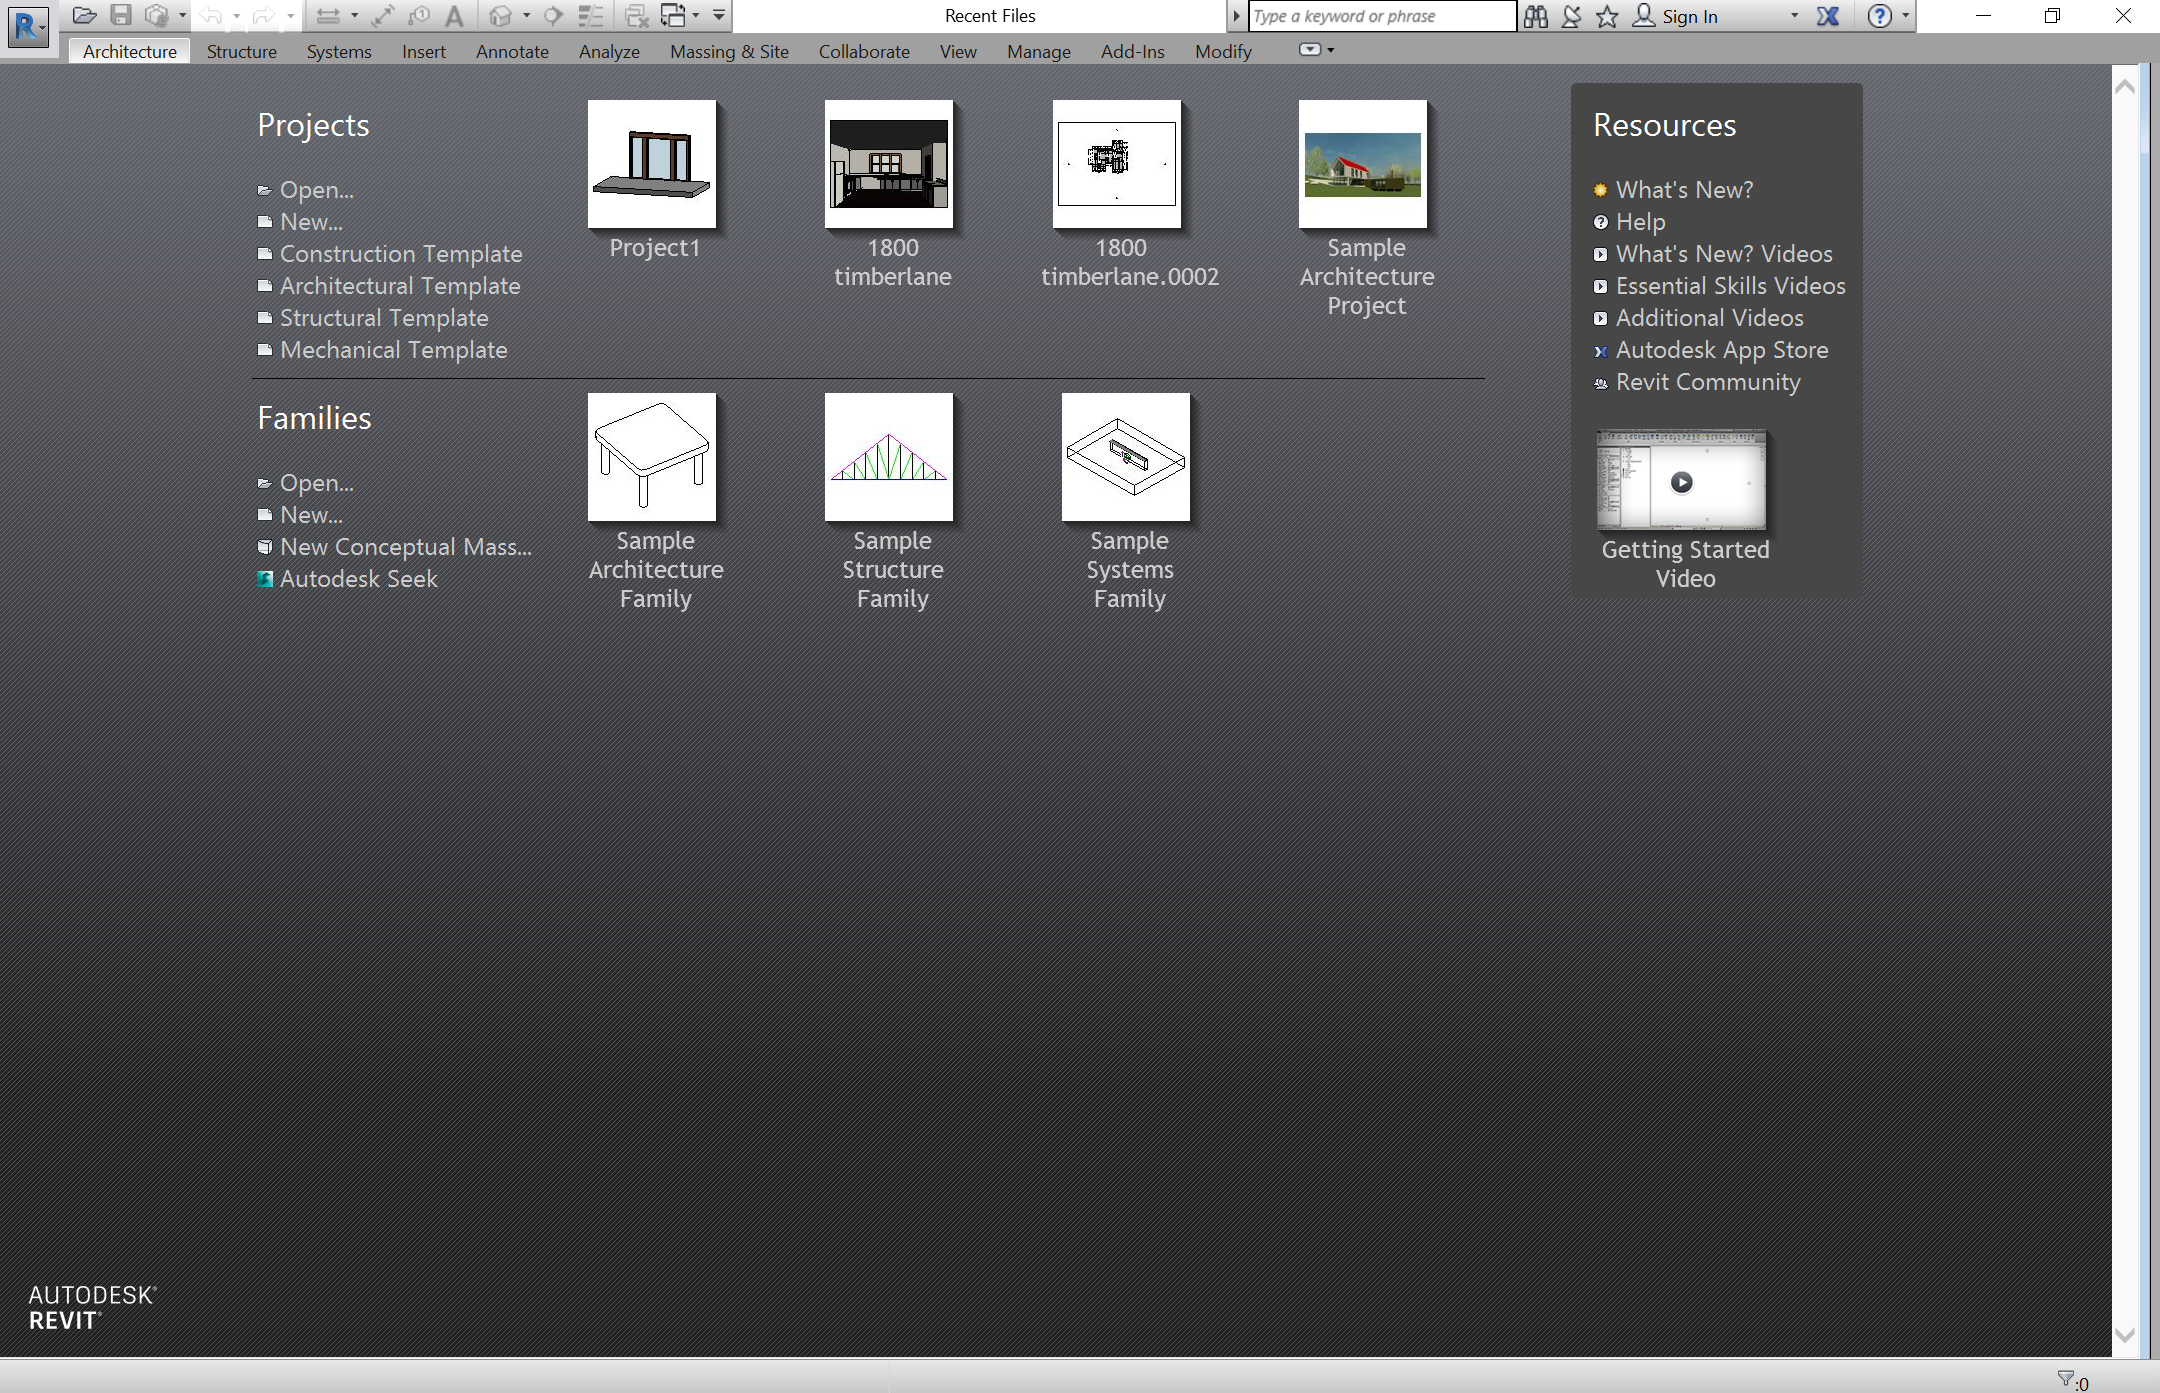
\includegraphics[width=\linewidth]{revitmainscene.PNG}
	\caption[The revit start page]{This figure shows the opening page when you open up the Revit Application.}
	\emph{There are three major parts to the Revit Application Main Page.}
	\label{fig:revmainscene}
\end{figure}
\begin{marginfigure}
	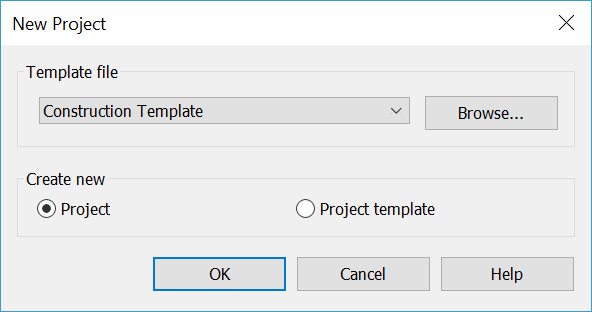
\includegraphics[width=\linewidth]{revitnewfile.png}
	\caption[A revit New file popup]{This is new file popup, you see this whenever you wish to create a new project. You will always be creating a Project, not a Project Template.}
	\emph{You will not be creating any files with the Construction Template}
	\label{fig:revnewfile}
\end{marginfigure}


\newthought{Among the links} are: \menu{Open...} which opens an already existing project, and \menu{New...} which presents to you the process to create a new project, and various templates. The images and captions within the project section are existing projects that have been opened recently.



\newthought{We are going} to start a new project. If you click on \menu{New...} you should have a popup window like in Figure \ref{fig:revnewfile}. 

Once you click \menu{Browse...} you should be taken to another popup. The popup, which is shown in figure \ref{fig:revtmpview} has a list of templates used in Revit Projects. The template you will want to you is called \menu{default}. Once the template is selected click \menu{Ok} and be off onto the project.


\begin{figure}
	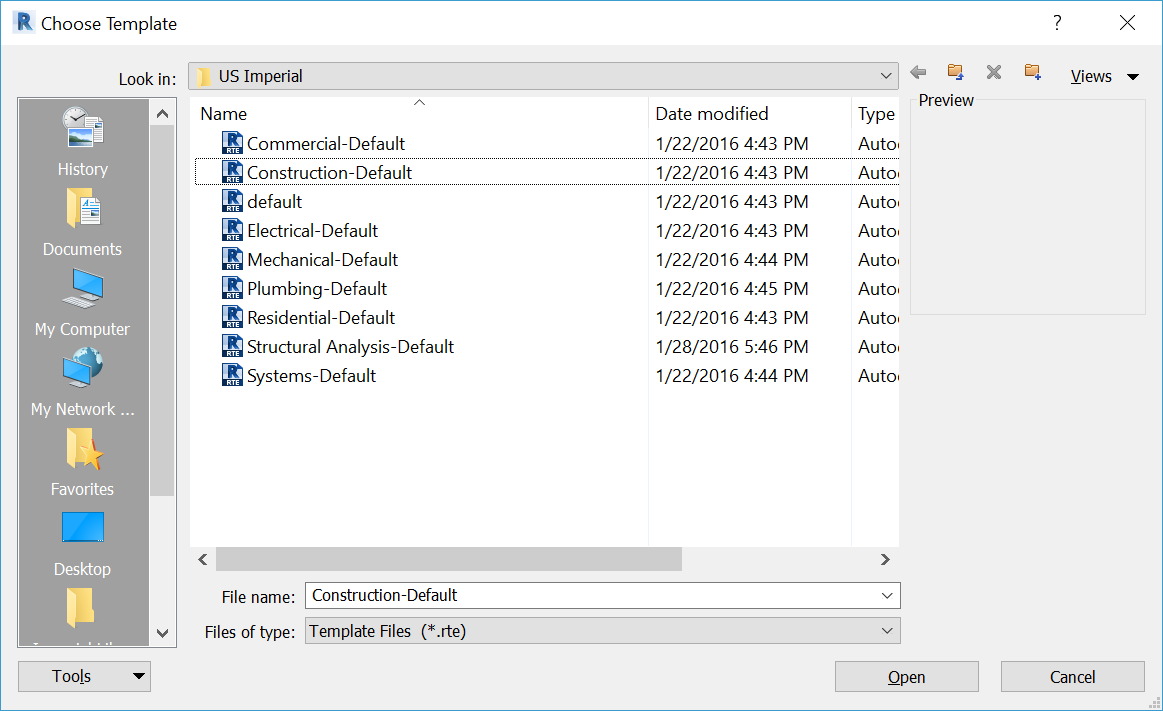
\includegraphics[width=\linewidth]{revittemplateview.png}
	\caption[A template file list]{A list of the templates that will popup on your screen}
	\label{fig:revtmpview}
\end{figure}
\marginnote{if you can't find it, the file path is: \directory{ProgramData / Autodesk / RVT 2016 / Templates / US Imperial / default}}

\begin{figure*}
	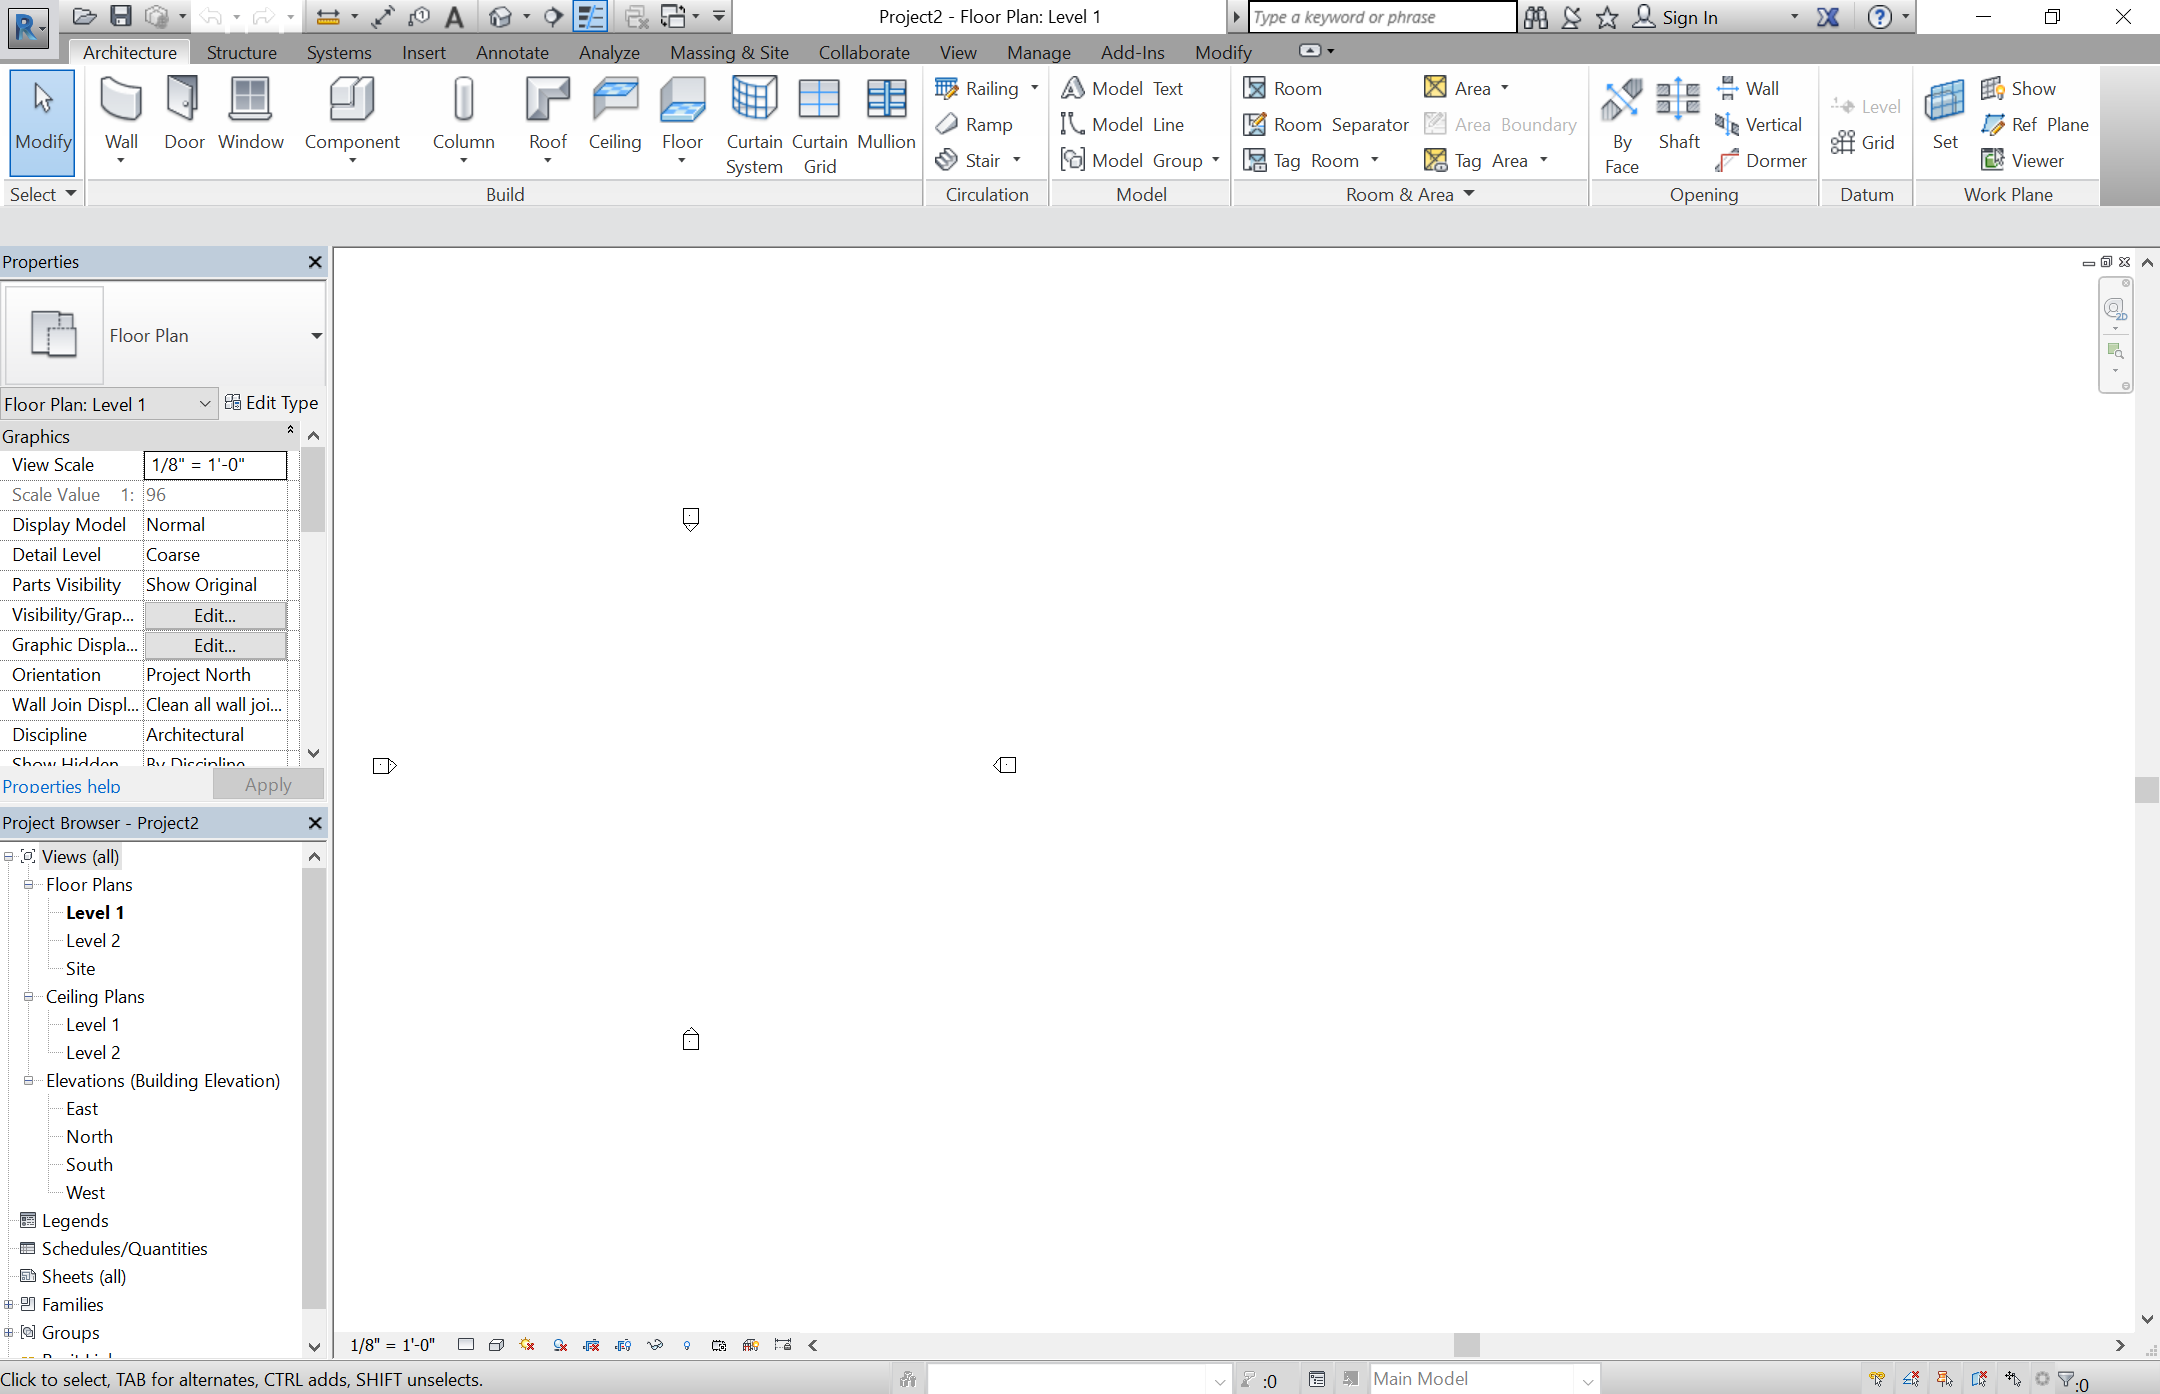
\includegraphics[width=\linewidth]{revitfullpageview.png}
	\caption[A revit default workspace]{A full screen example of the Revit workspace. Composed of multiple ribbon banners, and views. The large whitespace is the plane on which you  have your building}
	\label{fig:revfullview}
\end{figure*}

\clearpage
\section{Elements of the Revit Interface}

\begin{figure*}
	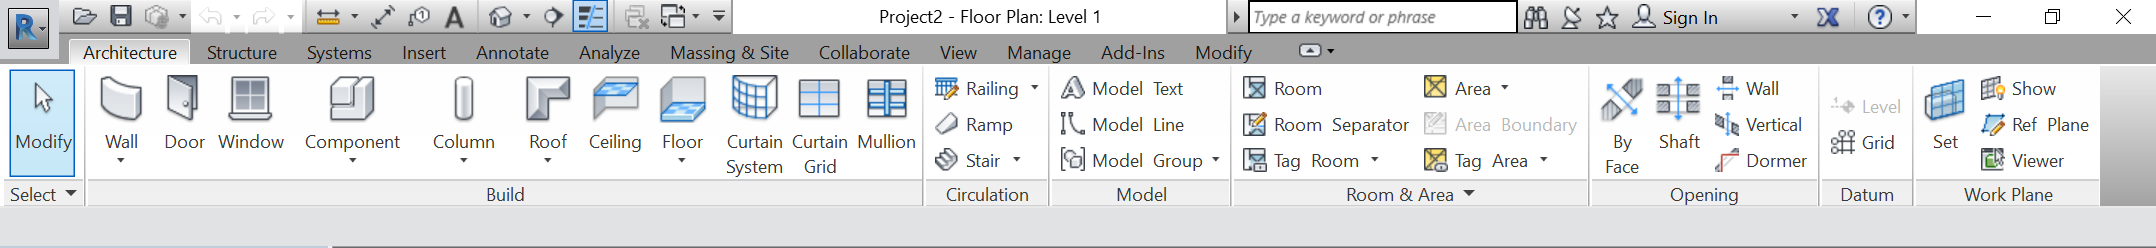
\includegraphics[width=\linewidth]{revittopbar.png}
	\caption[The revit top bar]{The revit top bar, at it's base.}
	\label{fig:revtopbar.png}
\end{figure*}

In the figure \ref{fig:revtopbar.png} you can see what we will refer to as the \menu{Top Bar}, this will be the location where all the tools of this program are located.

\marginnote{You won't be using the majority of these tabs, but it's smart to know what they do, along with the tools inside. See the Menu Tools sections reference for more. For the majority of this tutorial the only tabs will be: \menu{Architecture}, \menu{Annotate}, \menu{Massing \& Site}, \menu{View}, and \menu{Modify}} 
 
\newthought{You can see} icons for each tool, and above those is a line of tabs, called Ribbons, starting with \menu{Architecture}, then \menu{Structure}, \menu{Systems}, etc. When you click one of the ribbon labels you are taken to a new section of tools. 

As you create the house below, you will become familiar with all these tools; each tool is essential in the creation of a functioning model.

\newthought{The \menu{Architecture} tab}, which is show in Figure \ref{fig:revtopbar.png}, contains the tools to create the basic formation of a house: the foundation, the floors, the walls, and the windows.

\marginnote{Beware: overuse of the \mbox{\menu{Massing \& Site > Toposurface}}, and the \menu{Massing \& Site > Site Component} tools can lead to your computer becoming slow and sluggish.}

\newthought{The \menu{Annotate} tab} which is shown in the figure \ref{fig:revanntab} contains the tools which you use to markup the project. These tools document your creation, while also making presentation easier. They can be used to determine the size of your model, the angels of you walls, the width of you house for a variety of reasons.


\begin{figure*}
	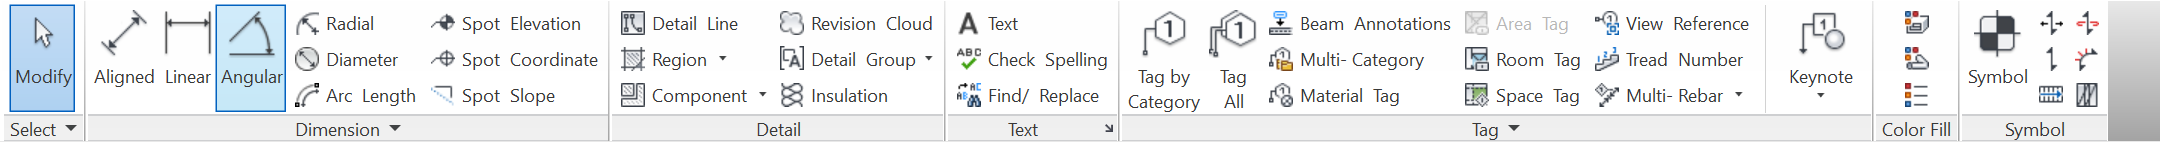
\includegraphics[width=\linewidth]{revitannotationbar.png}
	\caption[The annotation bar]{A picture of the \menu{Annotation} bar in revit.}
	\label{fig:revanntab}
\end{figure*}



\newthought{The \menu{Massing \& Site} tab}, in figure \ref{fig:revmastab} is used to model and map the terrain of your model.

\begin{figure*}
	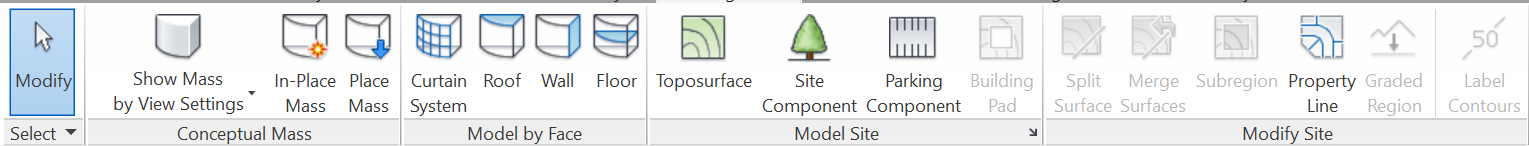
\includegraphics[width=\linewidth]{revitmassingsitebar.png}
	\caption[The massing and site bar]{A picture of the \menu{Massing \& site} bar in revit.}
	\label{fig:revmastab}
\end{figure*}


\newthought{The \menu{View} tab}, shown in figure \ref{fig:revviewtab}, contains essential tools for viewing and presenting your project. The \mbox{\menu{View > 3d View}} tool will become vital for visualizing your house in the future.


\begin{figure*}
	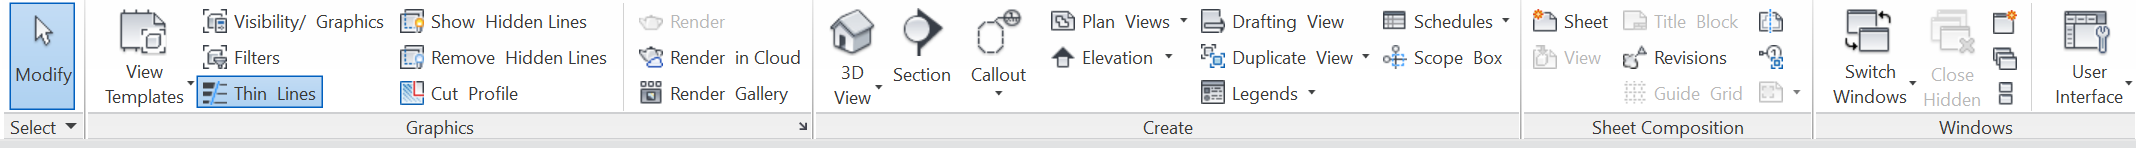
\includegraphics[width=\linewidth]{revitviewtab.png}
	\caption[The view bar]{A picture of the \menu{View} bar in revit.}
	\label{fig:revviewtab}
\end{figure*}

\newthought{The \menu{Modify} tab}, in figure \ref{fig:revmodtab}, is different from the others. While the previous tabs were meant to interact with the building, this tab is primarily focused on interacting with the objects that make the building up. For instance, splitting a singular wall is done inside the modify tab.

\begin{figure*}
	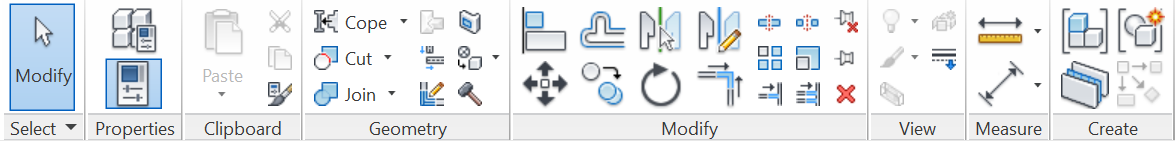
\includegraphics[width=\linewidth]{revitmodifytab.png}
	\caption[The modify bar]{A picture of the \menu{Modify} bar in revit.}
	\label{fig:revmodtab}
\end{figure*}






%------------------------------------------------


%----------------------------------------------------------------------------------------

\mainmatter

%----------------------------------------------------------------------------------------
%	CHAPTER 1
%----------------------------------------------------------------------------------------

\chapter{Chapter 1 - Creating Your House}
\label{ch:1}
Figure \ref{fig:revfinhouse} is a picture of what your house will look like.


\begin{marginfigure}
	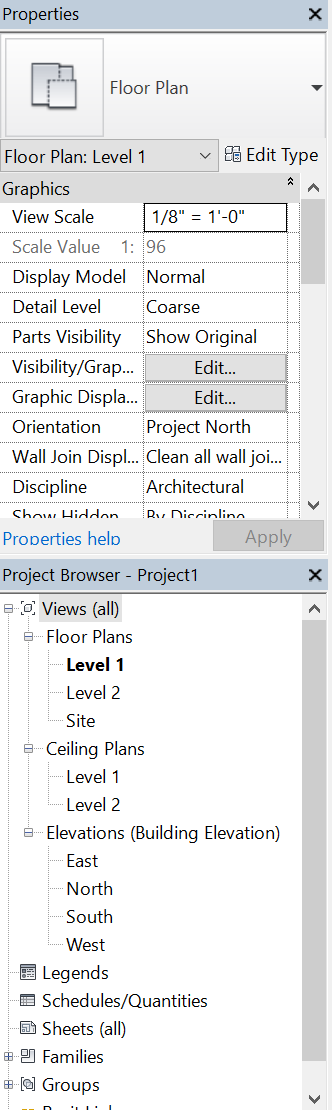
\includegraphics[width=\linewidth]{revitsidebar}
	\caption[The revit side bar]{A picture of the \menu{Revit Sidebar}}
	\label{fig:revsidebar}
\end{marginfigure}

\newthought{On the right} in figure \ref{fig:revsidebar}, you can see the \menu{Revit Sidebar}. This sidebar, which should be on the left hand of your revit window, is the detail window for everything you do. in the \menu{Revit Sidebar > Properties} you can see the type of object, and the specifications for it. in the \menu{Revit Sidebar > Project Browser} you can see a list of all the views and documents associated with your project.
 
%------------------------------------------------

\section{Selecting and Creating Elevations}
The following guide's purpose is to establish an understanding of altitudes and elevations in 3d architecture.
\begin{enumerate}

	\begin{marginfigure}
		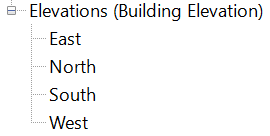
\includegraphics[width=\linewidth]{revitelevationslistview.png}
		\caption[The revit elevations list]{A view of the elevations: East, North, South, and West}
		\label{fig:revelevlistview}
	\end{marginfigure}
	
	\item Within \menu{Sidebar > Project Browser > Elevations} is the elevations list.
	\item Refer to figure \ref{fig:revelevlistview} and click on the \menu{Sidebar > Project Browser > Elevations > South} button
	\item You should see elevation lines in the main workspace. if you click along the line once, it will become like figure \ref{fig:revelevclick}, you should click and drag the leftmost circle to the right until the line becomes shorter.
	
	\begin{marginfigure}
		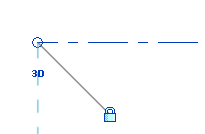
\includegraphics[width=\linewidth]{revitelevationsclick.png}
		\caption[Clicked elevation lines]{Elevation lines that have been clicked once}
		\label{fig:revelevclick}
	\end{marginfigure}
	
	\item Each elevation has two main elements, the name and the altitude. Generally your foundation should be several feet under the ground.
	\item You have two elevations currently: \menu{Level 1} and \menu{Level 2}
	\item You can either use your scroll wheel too zoom into the elevations, or you can use the keybinding: \keys{Ctrl + Z + F}
	\item If you click on the text of \menu{Level 1} where it says \menu{0'-0"} it will allow the input of a new altitude
	\item Click on the altitude of both \menu{Level 1} and \menu{Level 2} and change their altitudes
	
	\begin{itemize}
		\item For \menu{Level 1} where the altitude should be \menu{-14'0"}
		\marginnote{\menu{-4'0"} generally is a good altitude to keep your foundation base, \menu{Level 1} is the foundation for this house, for instance.}
		\item for \menu{Level 0} where the altitude should be \menu{10'0"}
	\end{itemize}
	
	\section{Creating additional elevations}
	\marginnote{A context menu is what happens when you right click, the first option should be cancel, in this case, the option you're looking for should be the 10th down}
	\item If you right click on the uppermost elevation, \menu{Level 2}, you should get a context menu, it should include the option: \menu{Create Similar}. If you click on that option it should select the \menu{Architecture > Level} tool which creates an annotation, but it also has the same selected options as the elevation you selected.
	\item If you look at Figure \ref{fig:revoptbar} you should see what is called the \menu{Options Bar}, on it you can see multiple options: \menu{Make Plan View} and \menu{Offset:} which equals \menu{0'0"}
	
	\begin{marginfigure}
		
\includegraphics[width=\linewidth]{revitoptionsbar.png}
		\caption[The revit options bar]{The options bar, which is mostly used to set chain settings and offsets}
		\label{fig:revoptbar}
	
	\end{marginfigure}
	
	\item To create an elevation that is \menu{10'} above \menu{Level 1} Change the \menu{Option Bar > Offset:} to equal \menu{10'0"} while \menu{Create Similar} is selected, and click from the leftmost point of \menu{Level 2} and drag to the rightmost point. Reference figure \ref{fig:revelevlinethree}
	
	\begin{figure}
		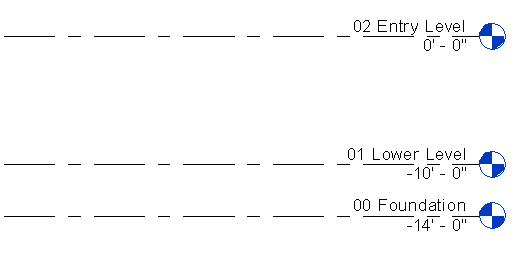
\includegraphics[width=\linewidth]{revitelevationlinethree.png}
		\caption[Shortened elevation lines]{When creating new elevations lines, you should drag from one end to the other to ensure consistency. In this case, \menu{Level 3} will be the level of entry, because its at a base altitude.}
		\emph{Make sure that your elevations look similar to this figure}
		\label{fig:revelevlinethree}
	\end{figure}
	
	\begin{marginfigure}
		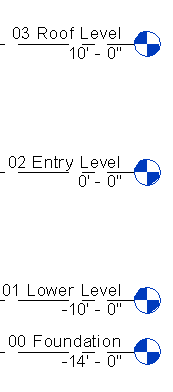
\includegraphics[width=\linewidth]{revitelevationsname.png}
		\caption[The names of elevation lines]{Make sure that your final elevations are named likewise}
		\label{fig:revelevname}
	\end{marginfigure}
	
	\item Use the same procedure as used to create \menu{Level 3} to create another elevation at \menu{10'0"}. To do this, make sure your \menu{Options Bar > Offset:} is set to \menu{10'} and create a similar elevation above \menu{Level 3}
	\item Similar in method to changing a elevation's altitude is changing an elevation's name. For instance, click on \menu{Level 1} where it says 'Level 1', so that it becomes a text box like when changing the altitude. Enter the following name: \menu{00 Foundation}
	\begin{itemize}
		\item Name the \menu{Level 1} this: \menu{00 Foundation}
		\item Name the \menu{Level 2} this: \menu{01 Lower Level}
		\item Name the \menu{Level 3} this: \menu{02 Entry Level}
		\item name the \menu{Level 4} this: \menu{03 Roof Level}
	\end{itemize}
\end{enumerate}

\chapter{Chapter 2 - Creating the Base of the House}
\label{ch:2}
The purpose of this guide is to instruct in the method of creating the foundation for the project.
\section{Creating the Retaining Walls}
\begin{enumerate}
	\marginnote{This is why we named our elevations the way we did in the previous chapter. Our floor plans are listed alphabetically in the \menu{Project Browser} so when we have the numbers preceding the name, they are both descriptive, and correctly ordered.}
	\item Select this view \menu{Sidebar > Project Browser > Floor Plans > 00 Foundation}
	\item Zoom into the lower right quadrant of the workspace
	\item From there, select the following tool: \menu{Architecture > Wall Tool}. When you click on the screen with this tool selected you create points, just like on a graph you click or drag another point out to create a line, or a wall in this case.
	\marginnote{It's good to make sure that your walls have the correct base and height. If the program does not let you select the correct height, while not perfect, another option is to choose unconnected for the \menu{Sidebar > Properties > Top Constraint} and then select the altitude for the elevation point, for instance, the offset would be \menu{10'0"} for \menu{02 Roof Level}}
	\item If you remember the \menu{Sidebar} for the interface explanation, there was \menu{Sidebar > Properties}, inside this is the options for the wall.
	
	
	\begin{tabular}{ c | c }
		Settings & \menu{Basic Wall Retaining - 12" Concrete}\\
		\hline
		Location Line & Wall Centerline\\
		Base Constraint & \menu{00 Foundation}\\
		Base Offset & \menu{0'0"}\\
		Top Constraint & Up to \menu{02 Entry Level}\\
		Top Offset & \menu{0'0"}\\
	\end{tabular}
	
	\item Click to create a base point, a line should begin to follow your cursor. You can easily create a wall by pointing your cursor in a direction, and typing in the distance.
	
	\begin{marginfigure}
		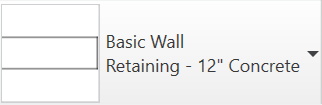
\includegraphics[width=\linewidth]{revitobjecttype.png}
		\caption[Revit object types]{When selecting an object in Revit. There is, of course, different object types. The image in this figure is the \menu{Object Selector}. For walls specifically, there are multiple types that we use. When referenced, the Object type can be explained as \menu{Sidebar > Properties > Object Selector > Basic Wall Retaining - 12" Concrete} or plainly as \menu{Basic Wall Retaining - 12" Concrete}}
		\label{fig:revobjtype}
	\end{marginfigure}
	
	\item create a base point and move your cursor to the left: type \keys{40'}
	\item If chain was selected in \menu{Option Bar > Chain:} then, you should just be able to move the cursor up and type in \keys{22'}, otherwise click on your last created point and repeat the aforementioned steps
	\begin{figure}
		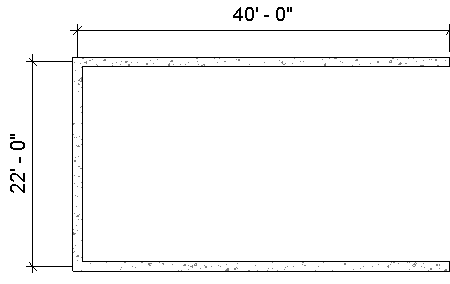
\includegraphics[width=\linewidth]{revitfoundationwalls.png}
		\caption{The foundation walls}
		\emph[Revit retaining walls]{This is what your walls should look like}
		\label{key:revfoundwalls}
	\end{figure}
	\item Repeat the same steps, moving your cursor right and typing: \keys{40'}
	
	
	
	\section{Creating your Foundation Walls}
	\item Select your retaining walls with the following options
	
	\newthought{}\begin{tabular}{ c | c }
		Settings & \menu{Basic Wall Foundation - 12" Concrete}\\
		\hline
		Location Line & Wall Centerline\\
		Base Constraint & \menu{00 Foundation}\\
		Base Offset & \menu{0'0"}\\
		Top Constraint & Up to \menu{01 Lower Level}\\
		Top Offset & \menu{0'0"}\\
	\end{tabular}
	
	\item Create the walls on the outside
	\begin{enumerate}
		\item select the rightmost edge of the bottommost wall with the wall tool selected
		\item Move the cursor to the right: type \menu{6'6"}
		\item Move the cursor up: type \menu{5'}
		\item move the cursor right: type \menu{10'6"}
		\item meet the intersect where the topmost point of your wall becomes directly right of the rightmost point of the top wall.
		\item Complete the walls by moving to the left until you hit the top wall.
	\end{enumerate}
	\item Figure \ref{fig:revfoundfinal} should be the final product of this level
	
	\begin{figure*}
		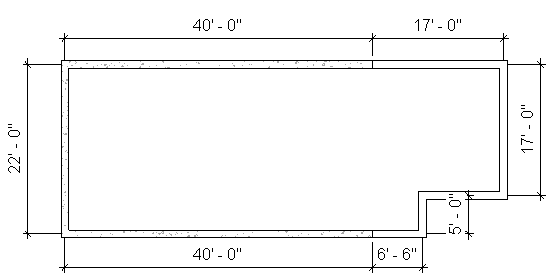
\includegraphics[width=\linewidth]{revitfoundationfinal.png}
		\caption[Revit foundation and retaining walls]{The final foundation walls}
		\emph{Make sure your walls  look like this}
		\label{fig:revfoundfinal}
	\end{figure*}
\end{enumerate}

\chapter{Chapter 3 - Creating the Terrain}
\label{ch:3}
The purpose of this guide is to introduce the basics of terrain creation in Revit. This should explain the basics of pads and terrain.
\section{Adding a Toposurface}
\begin{enumerate}
	\item Go to the following view: \menu{Sidebar > Project Browser > Floor Plans > Site}
	\item Select the following tool: \menu{Massing \& Site > Toposurface}
	\item Select the following options for \menu{Options Bar > Elevation:} to \menu{-0'6"}
	\item Add points to the left side of the building, like the figure \ref{fig:revtopoinit}
	\begin{figure}
		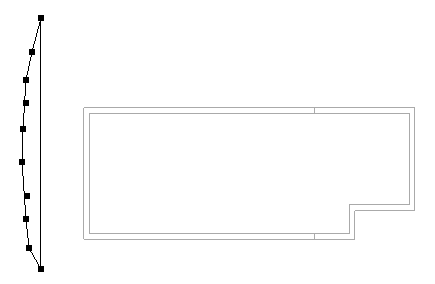
\includegraphics[width=\linewidth]{revittopographicinitial.png}
		\caption{Initial topographic points}
		\emph{Work to make sure yours looks similar, not exact}
		\label{fig:revtopoinit}
	\end{figure}
	\item Select the following options for \menu{Options Bar > Elevation:} to \menu{-10'}
	\item Select the points as in the figure \ref{fig:revtopotwo}
	\begin{figure}
		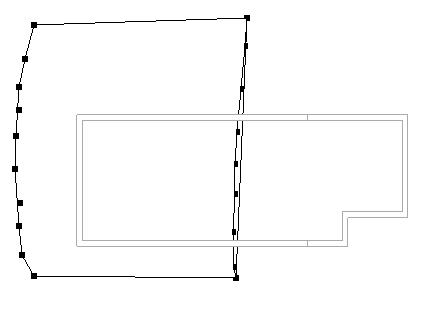
\includegraphics[width=\linewidth]{revittopographictwo.png}
		\caption{Second set of topographic points}
		\emph{Work to make sure yours looks similar, not exact}
		\label{fig:revtopotwo}
	\end{figure}
	\item Select the following options for \menu{Options Bar > Elevation:} to \menu{-11'}
	\item Select the points as in the figure \ref{fig:revtopothree}
	\begin{figure}
		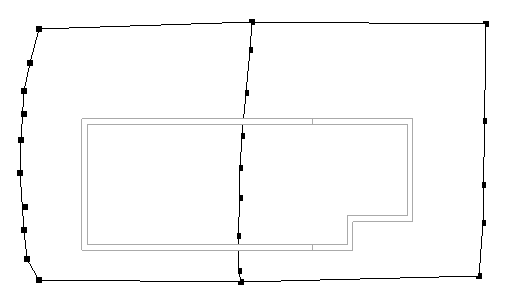
\includegraphics[width=\linewidth]{revittopographicthree.png}
		\caption{Third topographic points}
		\emph{Work to make sure yours looks similar, not exact}
		\label{fig:revtopothree}
	\end{figure}
	\clearpage
	\section{Setting up a Building Pad}
	\marginnote{Remember that it's best to avoid adding excessive amounts of topographic points, which may slow your computer.}
	\item Having finished the terrain surface by clicking the big green checkmark.
	\item To create a building pad click on each of the walls with the \menu{Massing \& Site > Building Pad} tool.
	\item Click each wall, finally click the purple line with three parallel lines attached: click it until the purples lines are only on the exterior of the walls. Reference figure \ref{fig:revtopopad}
	\begin{figure}
		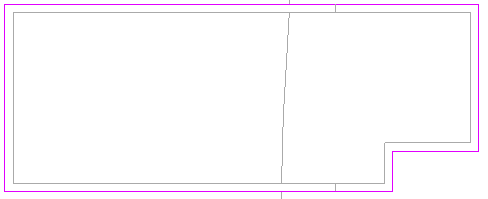
\includegraphics[width=\linewidth]{revittopographicpad.png}
		\caption[Building Pad Lines]{When building a pad, it's essential that it covers the buildings base, but doesn't extend past it. The pads purpose it to place a solid foundation base, while making sure that the terrain does not enter the floors of your building, so it removes any terrain where it's at.}
		\emph{Make sure your pad looks like this, it's not essential but recommended}
		\label{fig:revtopopad}
	\end{figure}
	\section{Creating a 3D view}
	\item Click on the tool \menu{View > 3d View}, it will create a new view called \menu{Sidebar > Project Browser > 3d Views > \{3D\}} right click on this view to rename it to something, I recommend \menu{To Building}
	\begin{marginfigure}
		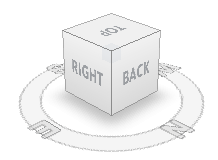
\includegraphics[width=\linewidth]{revitthreedviewcube.png}
		\caption[Revit 3D Maneuvering Square]{Use the 3d viewcube to move around the 3D environment. If you grip the sides and corners with your mouse, you can drag it to change your view. }
		\emph{The proficient use of this is essential, so make sure you focus on it in later projects.}
		\label{fig:revthreemansquare}
	\end{marginfigure}
	\item select your renamed \menu{3d View} and use the 3D maneuvering square to change the view. Reference Figure \ref{fig:revthreemansquare}
	\begin{figure}
		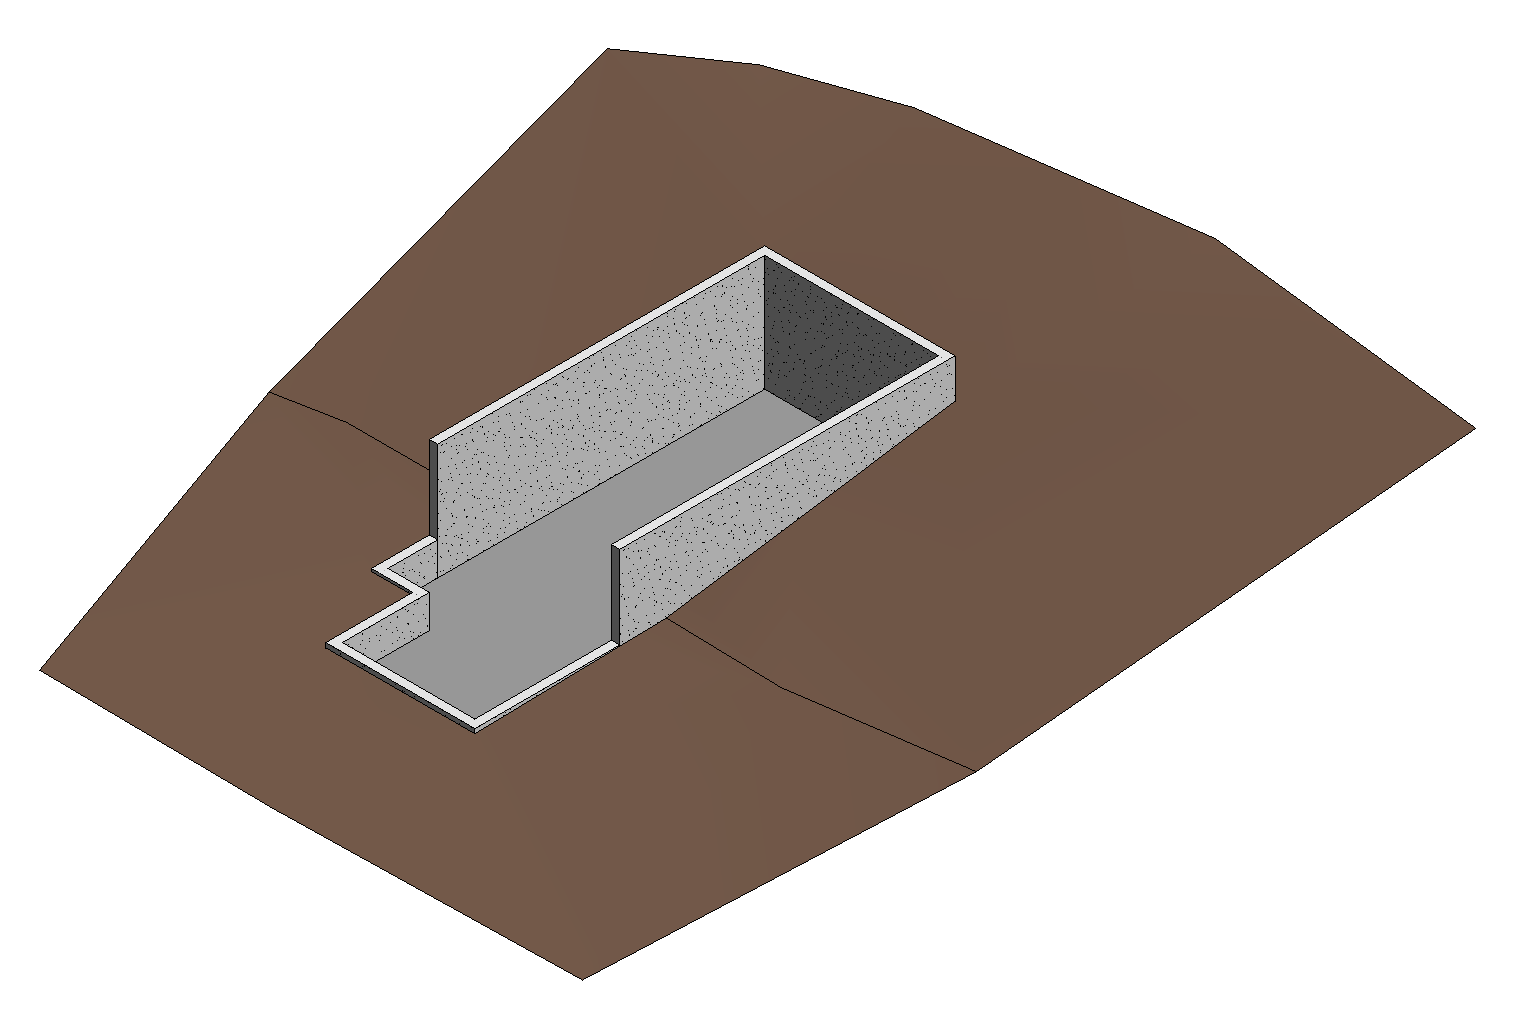
\includegraphics[width=\linewidth]{revitthreedtopographic.png}
		\caption[Revit 3D view after Topographic Creation]{It's Important that everything looks realistic. When presenting your building, you want to an accurate representation of what it would look like. If you wish for further information, either ask your teacher, or reference any information on rendering}
		\emph{Make sure your 3D view looks rather similar to this, but it will vary from person to person}
		\label{fig:revthreedtopo}
	\end{figure}
\end{enumerate}
	
\chapter{Chapter 4 - Creating Exterior Walls, Floors, and Roofs}
\label{ch:4}
The purpose of this guide is to continue on the education of wall creation. This also touches on the creation of wall retained floors, and non retained floors.
\section{Creating Exterior walls}
\subsection{Add walls to the entry level}

\begin{enumerate}
	\item go to the following view: \menu{Sidebar > Project Browser > Floor Plans > 00 Entry Level}
	\item Create the following walls with these options:
	
	\marginnote{If you are having issues with seeing objects below the current view level, then change the following settings. While you have the view selected in the \menu{Sidebar > Properties} there is an option called \menu{View Range}, if you go into that setting and change the \menu{View Depth > Level:} option to the appropriate level you wish to have your view depth to.}
	
	\newthought{}\begin{tabular}{c | c}
		Settings & \menu{Generic - 6"}\\
		\hline
		Location Line & Core Face Interior\\
		Base Constraint & \menu{02 Entry Level}\\
		Base Offset & \menu{0'0"}\\
		Top Constraint & Up to \menu{03 Roof Level}\\
		Top Offset & \menu{0'0"}\\
	\end{tabular}
	
	\item beginning at the bottom right, trace the interior of the three existing retaining walls, the three rightmost walls, by selecting endpoints. Reference figure \ref{fig:reventlvlwalls}.
	
	\begin{figure}
		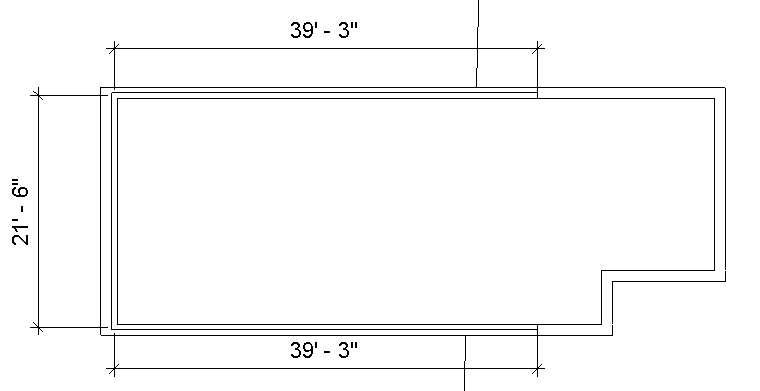
\includegraphics[width=\linewidth]{revitentrylevelwalls.png}
		\caption[Entry level walls]{The walls along the retaining walls which reach the exterior walls are meant to border the interior of the retaining walls. By selecting \menu{Core Face Interior} the walls are more easily alinged with the interior face of the walls.}
		\emph{Make sure your walls look like this, annotations excluded}
		\label{fig:reventlvlwalls}
	\end{figure}
	
	\subsection{Add walls to the Lower level}
	\item Open up the following: \menu{Sidebar > Project Browser > Floor Plans > 01 Lower Level}
	\item Use the following settings:
	
	\newthought{}\begin{tabular}{c | c}
		Settings & \menu{Generic - 6"}\\
		\hline
		Location Line & Core Face Interior\\
		Base Constraint & \menu{01 Lower Level Level}\\
		Base Offset & \menu{0'0"}\\
		Top Constraint & Up to \menu{03 Roof Level}\\
		Top Offset & \menu{0'0"}\\
	\end{tabular}
	
	\item Trace the interior of the Foundation walls, the 5 leftmost walls. Reference figure \ref{fig:revlowlvlwalls}
	
	\begin{marginfigure}
		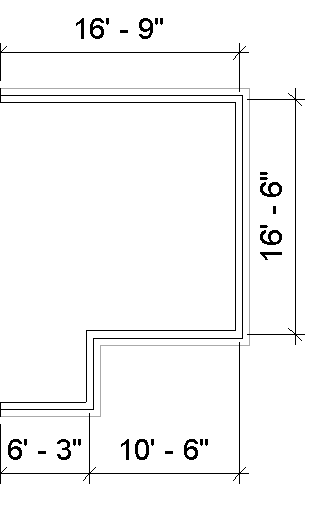
\includegraphics[width=\linewidth]{revitlowerlevelwalls.png}
		\caption{Lower Level Walls}
		\emph{Make sure your walls look like this, annotations excluded}
		\label{fig:revlowlvlwalls}
	\end{marginfigure}
	
	\clearpage
	
	\begin{figure*}
		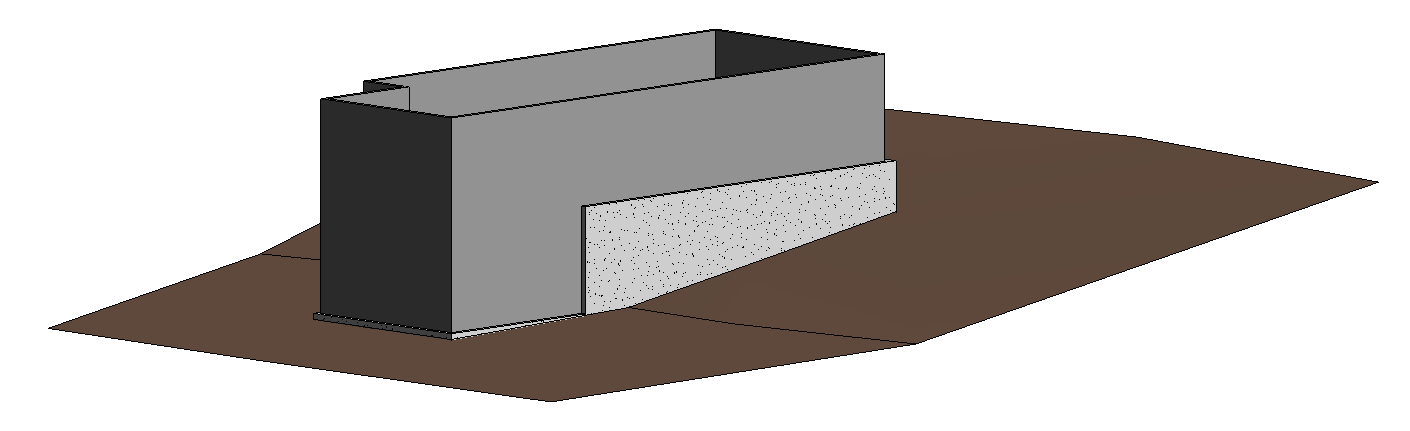
\includegraphics[width=\linewidth]{revitthreedouterwalls.png}
		\caption[Exterior walls 3D view]{This is the 3D view of the outer walls. If one of your walls is taller or shorter than the other, make sure that you have the correct height selected in your wall options.}
		\emph{Your 3D view should now look rather similar to this}
		\label{fig:revthreedoutwalls}
	\end{figure*}
	
	\section{Creating a Roof}
	\item Go to the following view: \menu{Sidebar > Project Browser > Floor Plans > 03 Roof Level}
	\item the tool you should use is called: \menu{Architecture > Build > Roof}
	\item The Roof should have the following settings in \menu{Sidebar > Properties}:
	
	\newthought{}\begin{tabular}{c|c}
		Settings & \menu{Basic Roof Generic - 12} \\
		Base offset & \menu{0'0"} \\
		Rafter Cut & Plumb Cut \\
		Slope & 1" / 12" \\
	\end{tabular}
	
	\subsection{Draw a roof line}
	
	\item When you select the roof tool, you are brought to the modify tab, you will want to select the line tool, which is under \menu{Modify | Create Roof Footprint > Draw > Line Tool}. Selecting that tool allows you to create a roof in the same was as a wall, except to create a roof, you must create a closed perimeter with your lines to define the roof.
	\item Make sure the option: \menu{Options Bar > Chain:} is not checkmarked, this means that when you click to create two points, it automatically starts to make the next points. 
	\item Make sure the option: \menu{Options Bar > Defines Slope:} is checkmarked. This means that the future slope that you have will be based on this side of the roof.
	
	\begin{marginfigure}
		
\includegraphics[width=\linewidth]{revitroofintersect.png}
		\caption[Revit Roof Intersection]{when you push a line past a walls end, it will give you guides in relation to other objects in the project. So for this one, you will want to click only when it gives you guide lines that reach to the rightmost wall.}
		\label{fig:revroofinter}
	\end{marginfigure}
	
	\item Trace the southernmost walls past the end, where it becomes parallel with the endpoints of the rightmost wall. The intersection should look like Figure \ref{fig:revroofinter}
	
	\subsection{Draw an offset roof line}
	
	\item As you did when creating an elevation line, to create a roof line that is offset from the roof\index{roof}, you will want to select an offset.
	\item Select the option for your wall line: \menu{Options Bar > Offset:} should equal \menu{-3'0"} as well as make sure that \menu{Options Bar > Defines Slope:} is not checked for the remaining lines.
	
	\marginnote{Be sure when creating any object with an offset that the result is indeed offset from the initial line that you placed. Failing to realize this and fix the error just means more work for you.}
	
	\item On your workspace, click on the last point you made and travel upward until you hit the top edge of the leftmost wall.
	\item Travel to the left until you hit the rightmost part of the to wall. 
	\item Travel down until your last line is perpendicular with your first. 
	\item Make your \menu{Options Bar > Offset:} to be \menu{0'} and connect the lines together, reference Figure \ref{fig:revrooflines} for an idea of what the finished product should be 
	
	\begin{figure}
		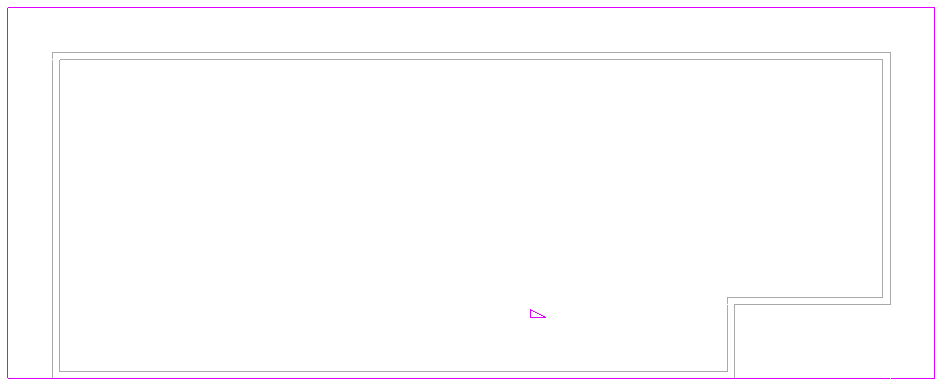
\includegraphics[width=\linewidth]{revitrooflines.PNG}
		\caption[Finished Roof Lines]{Your finished roof lines should be a singular line with define slope right against the southern wall. the rest of the lines should be offset \menu{3'0"} all along the wall}
		\emph{Make sure that your roof looks exactly like this, or at least similar}
		\label{fig:revrooflines}
	\end{figure}
	
	\section{Creating Floors}
	\subsection{Creating Lower Level Floors}
	\item Open up the view: \menu{Side Bar > Project Browser > Floor Plans > 01 Lower Level}
	\item Select the \menu{Architecture > Floors} tool, which you use to make floors, unsurprisingly
	
	\begin{marginfigure}
		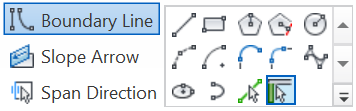
\includegraphics[width=\linewidth]{revitfloortool.png}
		\caption[Revit Pick Walls Tool]{The tool you are using to create a floor is specifically made to fill a room or a certain amount of rooms by selecting the boundaries of the floor based on the surrounding walls.}
		\emph{Make sure you are using the tool with the surrounding marquee}
		\label{fig:revfloortool}
	\end{marginfigure}
	
	\item The default tool selected should be sufficient, make sure you have the right tool selected, it's the \menu{Modify | Create Floor Boundary > Draw > Pick Walls} tool, check figure \ref{fig:revfloortool}
	\item Click all the walls in \ref{01 Lower Level}. This should be the same method as creating the building pad, except make sure that the lines are all interior rather than exterior.
	
	\begin{figure}
		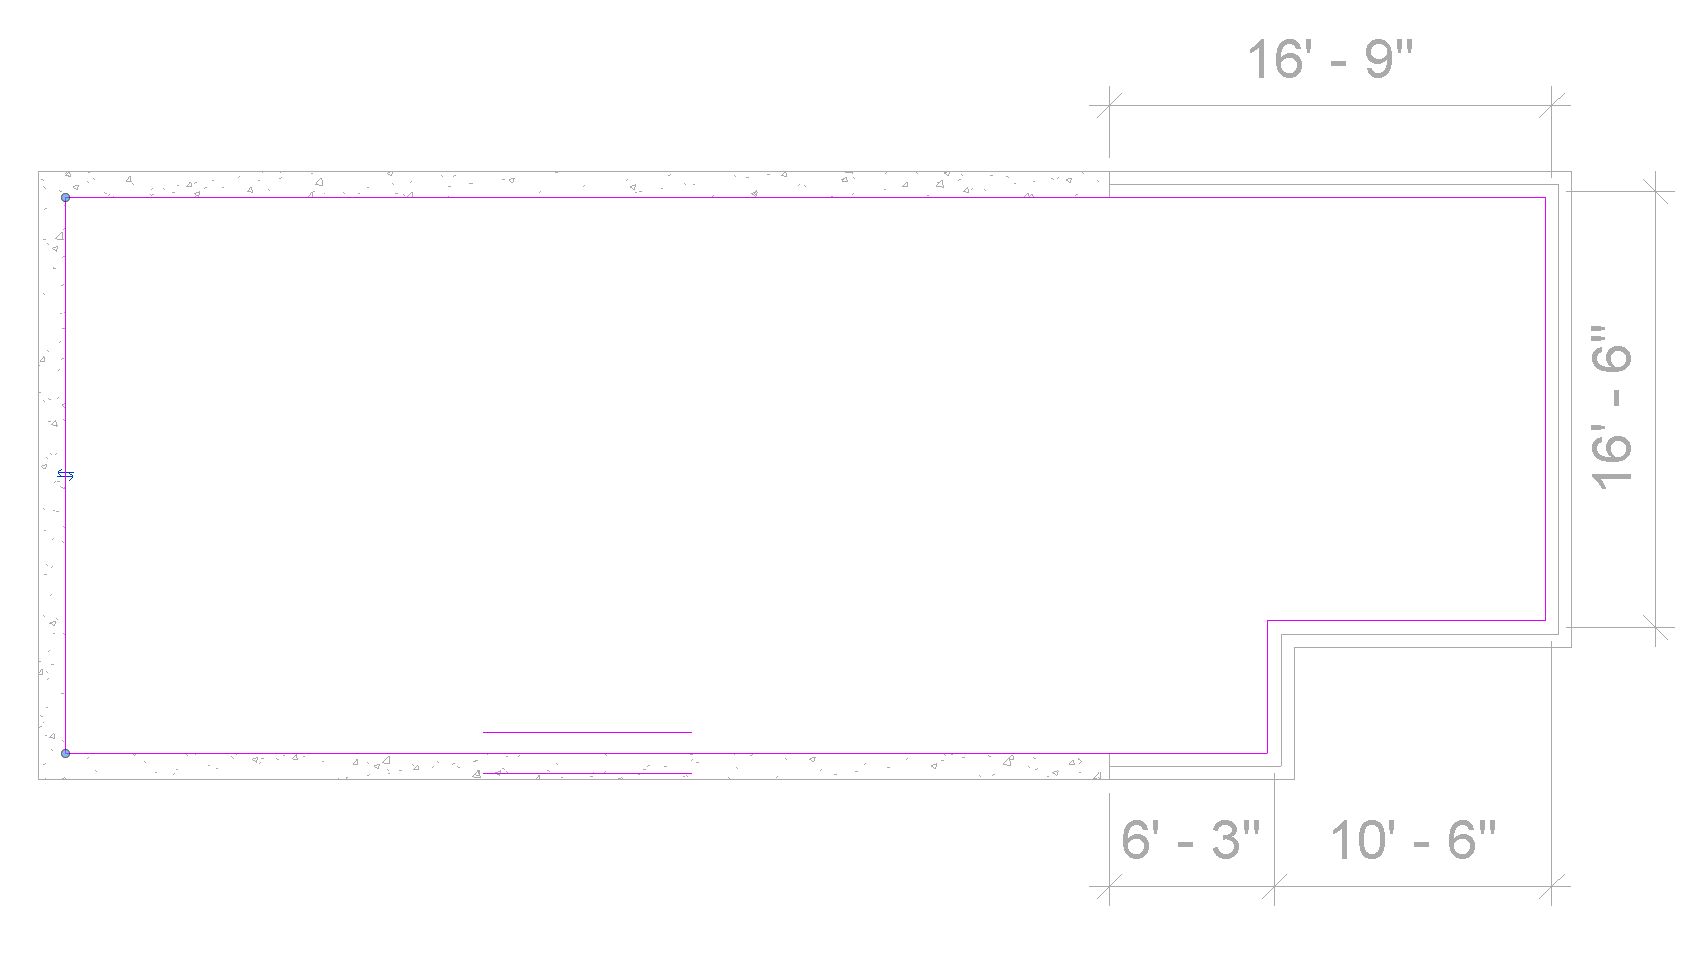
\includegraphics[width=\linewidth]{revitlowerlevelfloor.png}
		\caption[Lower level floors]{This should be the lower level floors, which are represented by the purple line. Make sure that the purple line is only on the interior}
		\emph{Make sure yours looks exactly like this, or similar.}
	\end{figure}
	
	\marginnote{The popups are in regards to the wall's geometry that you attach too. You will most likely never need to worry about that.}
	\item Say no to all popups after creating the floor, for the time being, you do not need to worry about those
	\subsection{Creating the Entry Level Walls}
	\item The creation of the \menu{01 Entry Level} walls is a bit more hands on.
	\item Navigate to \menu{Side Bar > Project Browser > Floor Plans > 01 Entry Level}.
	\begin{marginfigure}
		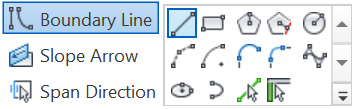
\includegraphics[width=\linewidth]{revitupperfloortool.png}
		\caption{Entry Level Floor Tools}
		\emph{Make sure you are using this tool, not the previous one.}
		\label{fig:revupperlevelfloortool}
	\end{marginfigure}
	\item Instead of the tool you were using before, select the \menu{Line Tool}
	\item Make sure that \menu{Options Bar > Chain:} is selected
	\item From the top right place a point to create the flooring
	\item Use the following method to create the Entry Level floors
	\begin{enumerate}
		\item Move to the right and type: \menu{36'}
		\item Move down and type: \menu{16'6"}
		\item Move to the right and type: \menu{25'}
		\item Move down and type: \menu{4'6"}
		\item Then move your cursor to the bottom left of the model and complete the sketch
	\end{enumerate}
	\begin{figure}
	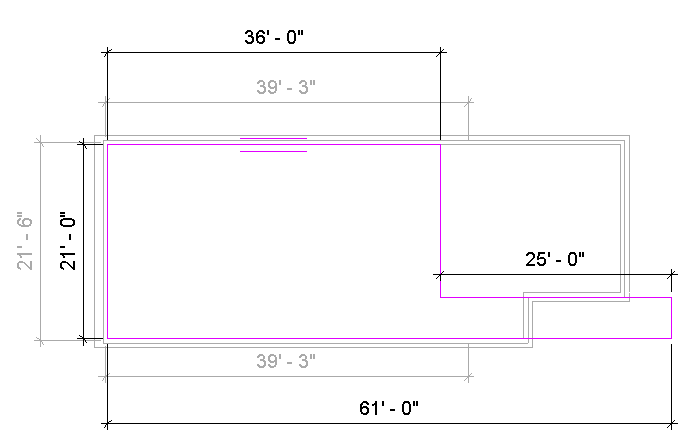
\includegraphics[width=\linewidth]{revitupperlevelfloors.png}
	\caption[Entry Level final floors]{The flooring for the Entry Level is essential. The fact that it doesn't fully cover that level is for the creation of a single atrium for the living room. As you get further you will see how the windows and stairs coincide with this design.}
	\emph{Your Floor should look, exactly like, or similar to this.}
	\end{figure}
	\item Once you have done this, you may finish the floorplan by clicking the large green checkmark
	\marginnote{Like before, any alert dialogs that pop up on the screen are not relevant to you, and should be either ignored or,if particularly concerning, consult your instructor.}
	
	\subsection{Viewing Your Floors in 3d}
	\begin{marginfigure}
		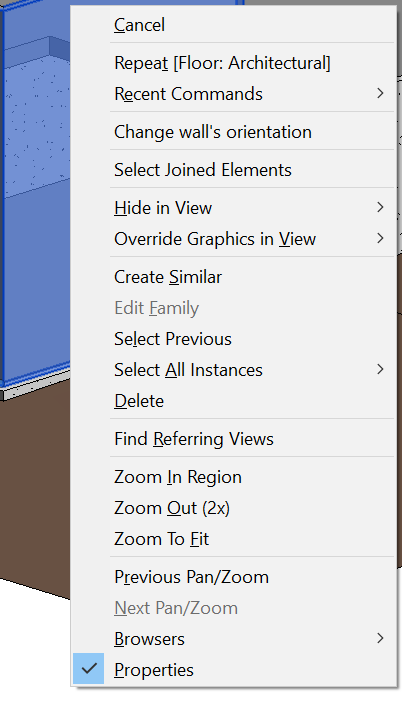
\includegraphics[width=\linewidth]{revit3dfloorcontext.png}
		\caption[3D wall context menu]{What pops up here should be the caption menu when right clicking a wall. }
		\label{fig:revthreedfloorcontx}
	\end{marginfigure}
	\item Select the view:\\ \menu{Side Bar > Project Browser > 3D Views > [What you named your primary 3D View]}
	\item Now, using your 3D view wheel, position your building do the front-right corner is at the forefront, this should be the default position
	\item, Right click the wall on the right: click on the context menu that comes up. Use the following options: \menu{Context Menu > Hide in View > By Element}
	\begin{figure}
		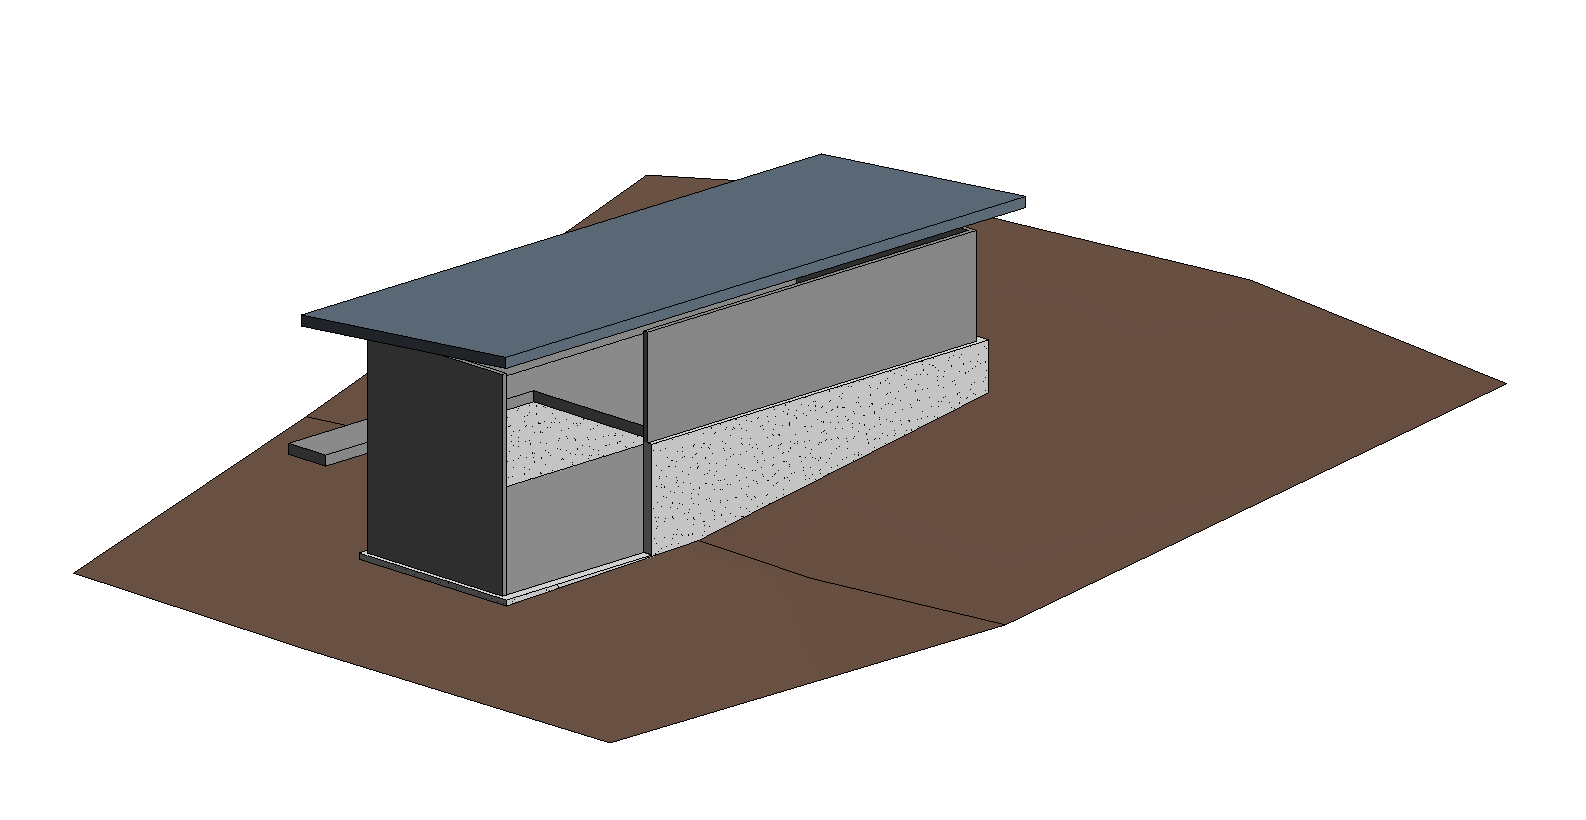
\includegraphics[width=\linewidth]{revit3dfloorview.png}
		\caption{The final 3d floor view}
		\emph{Your view should look similar to this, excluding view point discrepancies.}
		\label{fig:revthreedfloorfinal}
	\end{figure}
	\item Reference the Figure \ref{fig:revthreedfloorfinal}, for a final look at what your 3d view should look like
	 
\end{enumerate}

\chapter{Chapter 5 - Creating Interior Walls}
\label{ch:5}
In this guide you will continue on your education of wall creation. This time in the perview of interior wals.
\section{Creating Lower Level Interior Walls}
\begin{enumerate}
	\item Open up the following view: \menu{Side Bar > Project Browser > Floor Plans > 01 Lower Level}
	\item Use the following options for your wall properties
	
	\newthought{}\begin{tabular}{c | c}
		Settings & \menu{Generic - 6"}\\
		\hline
		Location Line & Wall Centerline\\
		Base Constraint & \menu{01 Lower Level Level}\\
		Base Offset & \menu{0'0"}\\
		Top Constraint & Up to \menu{02 Entry Level}\\
		Top Offset & \menu{0'0"}\\
	\end{tabular}
	
	\item Add walls:
	\begin{enumerate}
		\begin{marginfigure}
			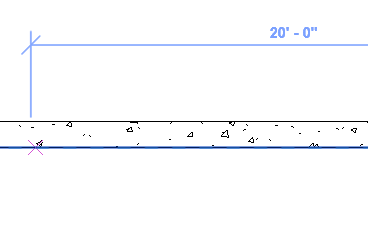
\includegraphics[width=\linewidth]{revitwalldistance.png}
			\caption{Wall distance guide}
			\emph{It should look like this when you click}
			\label{fig:revwalldist}
		\end{marginfigure}
		\item Beginning at the far left wall, move your cursor until the guide states that you are \menu{20"0'} away from the right corner wall. Look at the figure \ref{fig:revwalldist} to determine how it should look when you click.
		\item Create a wall perpendicular to that point, and bring it down until it reaches the far wall.
		\item At this point, refer to the figure \ref{fig:revlowerlevelwallsfinal} to continue the walls on this level. It is not essential that your walls are exactly the same.
		\begin{figure}
			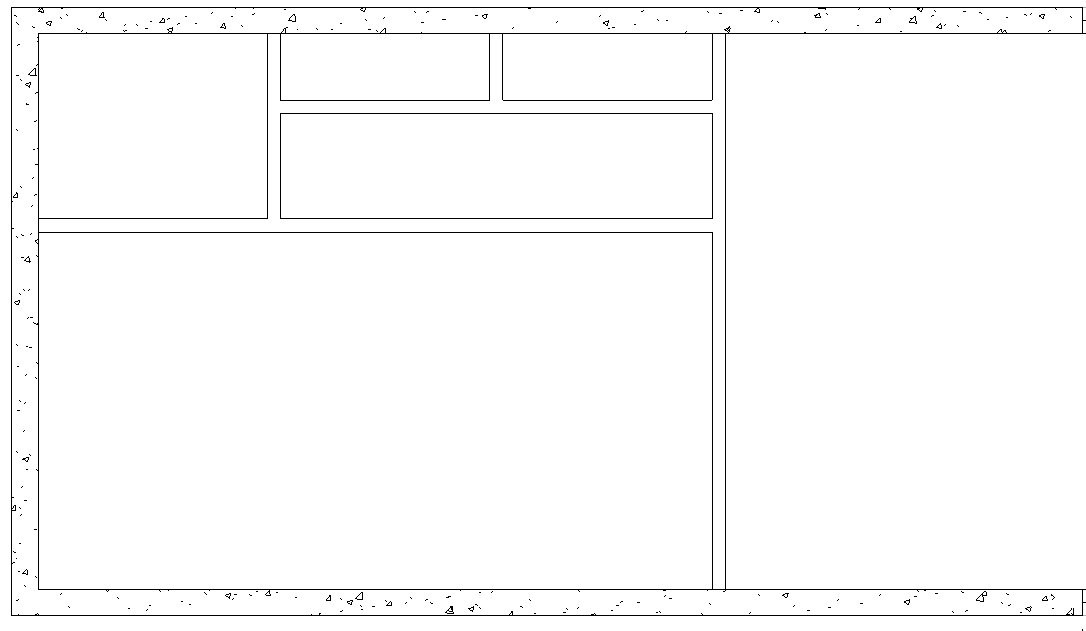
\includegraphics[width=\linewidth]{revitlowerlevelwallsfinal.png}
			\caption{The lower level walls guide}
			\emph{Your walls should look similar, but not exactly like this. All of this can be changed later of course}
			\label{fig:revlowerlevelwallsfinal}
		\end{figure}
		
		\begin{marginfigure}
			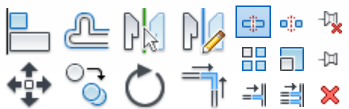
\includegraphics[width=\linewidth]{revitlowerlevelwallstools.png}
			\caption{The split tool selected}
			\label{fig:revlowerlevelmodtool}
		\end{marginfigure}
		\item You should use the \menu{Modify | Place Walls > Modify > Split Element} tool to split a point in the far right interior wall, to create a hallway.
		\item Select both end of the now split wall, to create the hallway. Check figure \ref{fig:revlowerlevelwallshallway} 
		\begin{figure}
			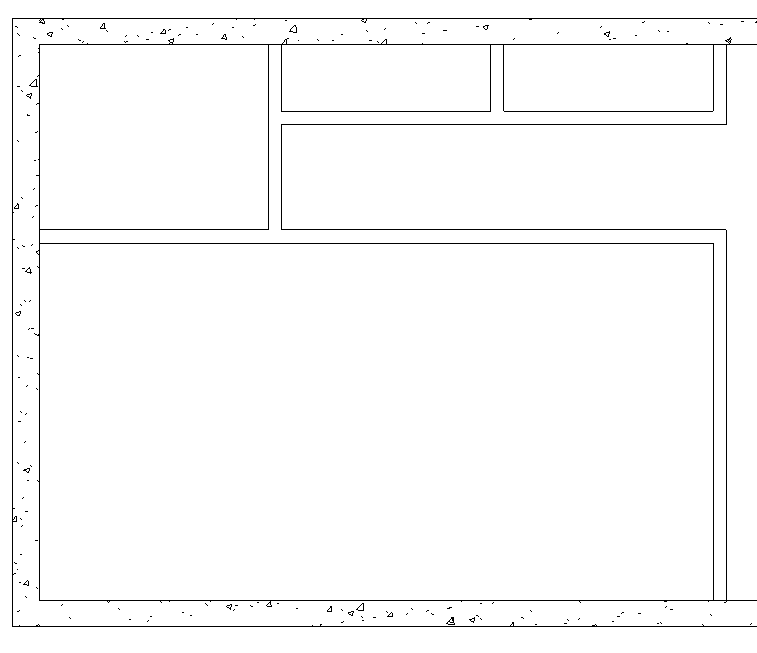
\includegraphics[width=\linewidth]{revitlowerlevelwallshallway.PNG}
			\caption{A completed hallway}
			\emph{Your hallway should look very similar, if not exact to this}
			\label{fig:revlowerlevelwallshallway}
		\end{figure}
	\end{enumerate}
	\section{Creating the Entry Level Walls}
	\item In this section, you're going to take charge on the construction of the Entry Level walls, following a figure. This should be on view: \menu{Side Bar > Project Browser > Floor Plans > 02 Entry Level}, and using the following options:
	
	\newthought{}\begin{tabular}{c | c}
		Settings & \menu{Generic - 6"}\\
		\hline
		Location Line & Wall Centerline\\
		Base Constraint & \menu{02 Entry Level}\\
		Base Offset & \menu{0'0"}\\
		Top Constraint & Up to \menu{03 Roof Level}\\
		Top Offset & \menu{0'0"}\\
	\end{tabular}
	
	\marginnote{Advanced: When you are creating your Entry Level walls, if you have trouble seeing because you are seeing the lower level walls at fulltone, do this: To select multiple walls for an options hold down the \keys{Ctrl} key and click the lowerlevel walls that you want to be halftone. When those are selected, rightclick on one of them, and click \menu{Context Menu > Override Graphics in View > Element}, a popup should come onto your screen. in the top right corner of that popup is a checkbox that says \menu{Halftone:} if you check that and click apply, then it will be halftone}
	\item In the figure \ref{fig:revuppwallsfinal} you should be creating the walls that are not halftone, meaning the walls that are the darker shade.
	
	
	\begin{figure*}
		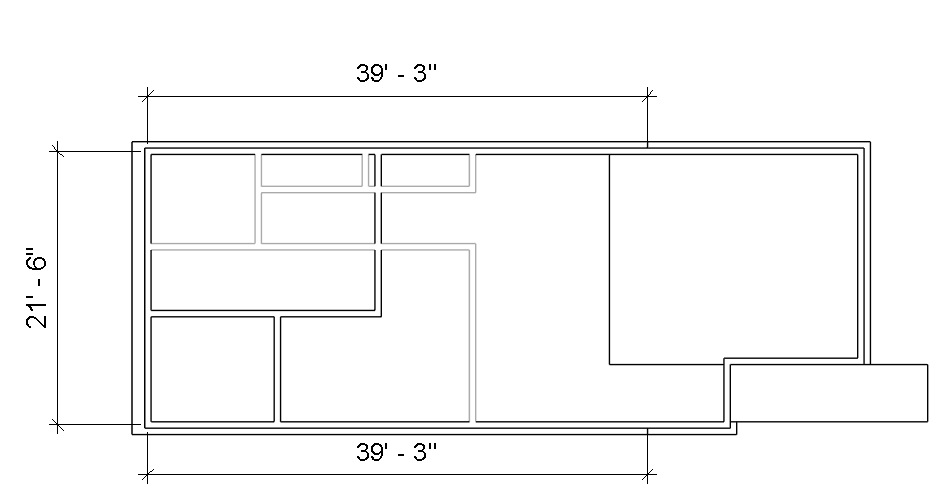
\includegraphics[width=\linewidth]{revitupperfloorsfinal.PNG}
		\caption{Entry Level interior walls}
		\emph{You can change these up however you want, but make sure they have similar composition}
		\label{fig:revuppwallsfinal}
	\end{figure*}
	
	\item When you are done creating the walls, if you wish to remove the ability to see the lowerlevel walls while on that level, use this option while the white background is clicked: \menu{Side Bar > Properties > View Level > View Depth > Level:} and change the option to \menu{Associated Level}
\end{enumerate}

\chapter{Chapter 6 - Creating Doors and Windows}
\label{ch:6}
In this particular section, you will be guided into adding Doors and Windows, which also doubles as a guide to the initial selection of objects
\section{Adding Exterior Doors}
\begin{enumerate}
	\item Go to the view level: \menu{Side Bar > Project Browser > Floor Plans > 01 Lower Level}
	
	\subsection{Adding Objects from a Library}
		\item Have the door tool selected, which is: \menu{Architecture > Build > Door}
		\marginnote{The Tool: \menu{Model In-Place}, which is adjacent to \menu{Load Family} Allows you to create your own furniture right into the workspace. It is an advanced tool, but if you continue along the Revit path, you may come across that tool later}
		\marginnote{Assume that our document root of this example is: \directory{C: / Program Data / Autodesk / RVT 2016 / Libraries / US Imperial}}
		\item Inside the Modify bar is the following option: \menu{Modify | Place Door > Mode > Load Family} When you click on that, a popup with an object directory comes up
		\item Go into the following directory to find the required object: \directory{Doors > Double-Glass.rfa}. If you are unable to find it, you can substitute it with any other available model.
		\item A table should come up, this allows you to load in select objects in that door group, or all of them. Just click on the first cell of the table, which is \menu{68"x80"} and click \keys{OK}
	\subsection{Creating the Lower Level Exterior Door}
		\item After clicking OK, you should have the door selected. Place it on the bottom of the rightmost wall. When placing a door, the orientation that the door swings, is dependant on which side of the wall your mouse is closest to. You're going to want your mouse nearest to the right side of the wall. This will cause the door to swing out into the exterior. When referring to a doors orientation, we will refer to as an exterior or interior swing. If the door is inside, then the exterior is merely swinging outside the room that it is being placed.
		\begin{marginfigure}
			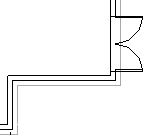
\includegraphics[width=\linewidth]{revitlowerexteriordoor.png}
			\caption{The Revit Lower Level Exterior Door}
			\emph{Your door should look similar to this, though the location doesn't have to be exact, it should be around the same area.}
			\label{fig:revlowerouterdoor}
		\end{marginfigure}
		\item We can refer to this door in the same way as walls we placed earlier, using the following options table, as well as choosing different doors like choosing different walls
		
		\newthought{}\begin{tabular}{c | c}
			Settings & \menu{Door-Double-Glass 68"x80"}\\
			\hline
			Sill Height & \menu{0'0"}\\
			Head Height & \menu{6'8"}
		\end{tabular}
	\subsection{Creating the Entry Level Exterior Door}
		\item Using the same door settings as before go to view: \menu{Side Bar > Project Browser > Floor Plans > 02 Entry Level}
		\begin{marginfigure}
			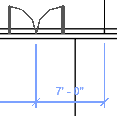
\includegraphics[width=\linewidth]{revitupperlevelexteriordoor.png}
			\caption [Entry Level Exterior Door] {Your door should be placed only when you see the \menu{7'0"} guide marker next to your door. This represents the distance to the end of the Retaining Wall. Remember that there is a difference between your Retaining and Foundation Walls, your retaining walls are meant to Retain Terrain.}
			\emph{Your door should look like this}
			\label{fig:revupperouterdoor}
		\end{marginfigure}
		\item Prepare to place the door on the topmost retaining wall. Only place it when the guide lines show that you are \menu{7'0"} away from the right edge of the retaining wall, reference Figure \ref{fig:revupperouterdoor}
		\item Load in an object like before, the directory is: \directory{Doors / Residential / Door-Interior-Single-Full Glass-Wood.rfa}. Select only the seventh cell down in the table and click \keys{OK}
		\begin{marginfigure}
			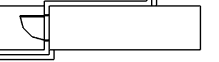
\includegraphics[width=\linewidth]{revitupperouterbalconydoor.png}
			\caption{The Balcony Door}
			\emph{Your door should look like this}
			\label{fig:revupperouterbalcdoor}
		\end{marginfigure}
		\item Using that door, place a door with an interior swing on the balcony. Refer to Figure \ref{fig:revupperouterbalcdoor}
	\section{Adding Interior Doors}
	\item Stay on the Floor Plan that you're currently on.
	\item Use the following door settings:
		\newthought{}\begin{tabular}{c | c}
			Settings & \menu{Single-Flush 30"x80"}\\
			\hline
			Sill Height & \menu{0'0"}\\
			Head Height & \menu{6'8"}
		\end{tabular}
	\subsection{Entry Level Interior Doors}
		\item There should be three identifiable rooms on the Entry Level: A Medium Sized Bedroom, A Closet, and Everything else.
		\item Click on the \menu{Medium Size Bedroom} on it's bottom right edge. Put an interior facing door near the right edge of the bottomost wall of that room.
		\item On the left side of that wall is the adjacent wall which the \menu{Medium Size Bedroom} shares with the \menu{Closet} Place an exterior facing door on the closets topmost wall
		\item Refer to Figure \ref{fig:revupperinterdoors} for an idea of what this means
		
		\begin{figure}
			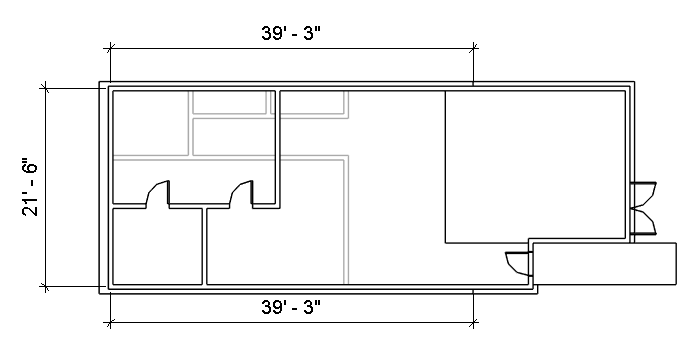
\includegraphics[width=\linewidth]{revitupperinteriordoors.png}
			\caption[Upper Interior Doors]{The Upper Interiors doors access these two rooms, you can see the door connecting the \menu{Medium Size Bedroom} and \menu{Everything Else} is interior because it's facing into the wall you're attaching it to. The closet door is exterior because it's facing away from the main room it's connecting. In an effort to stay away from pedantry, it's best to look at the following figure and then reference the guide for specific details. You'll get a hang of it}
			\label{fig:revupperinterdoors}
		\end{figure}
		
	\subsection{Lower Level Interior Doors}
		\item You should use the same door settings as the previous sub-section
		\item You should identify Five untique rooms: the \menu{Master Bedroom}, the smaller \menu{Closet 1}, the larger \menu{Closet 2}, The room which is larger than the closets, yet smaller than the Master Bed, the \menu{Bathroom}, and finally \menu{Everything Else}:
		\marginnote{You can safely assume that the main room is the first listed. So when it's exterior facing, we mean the exterior of the main room.}
		\begin{itemize}
			\item Place a door on the \menu{Closet 1} connecting to \menu{Everything Else}, exterior facing
			\item Place a door on the \menu{Closet 2} connecting to \menu{Everything Else}, exterior facing.
			\item Place a door on the \menu{Bathroom} connecting to \menu{Everything Else}, interior facing
			\item Place a door on the \menu{Master Bedroom} connecting to \menu{Everything Else}, interior facing.
		\end{itemize}
		\item Reference Figure \ref{fig:revlowerintwalls}
		\begin{figure}
			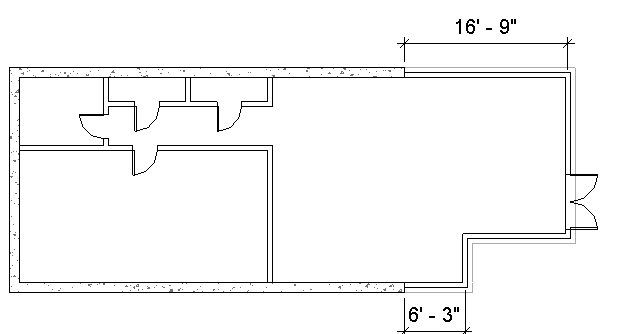
\includegraphics[width=\linewidth]{revitlowerlevelinteriorwalls.png}
			\caption{Lower Level Interior Walls}
			\emph{In this case, your doors do not have to look exactly like mine, although the orientation has to be correct. Look at the listing and see how the exterior and interior facing coincides with the picture. The leniency you have is, for instance, changing where you have the door of the \menu{Master Bedroom.}}
			\label{fig:revlowerintwalls}
		\end{figure}
	\section{Adding Windows}
	\subsection{Lower Level Windows}
		\item Open up this view: \menu{Side Bar > Project Browser > Elevations > South}
		\item Select the following tool; \menu{Architecture > Build > Window}
		\item Use the following properties:
		
		\newthought{}\begin{tabular}{c | c}
			Settings & \menu{Fixed 36"x48"}\\
			\hline
			Sill Height & \menu{3'0"}\\
			Head Height & \menu{7'0"} 
		\end{tabular}
		
		\item With the window selected, place it along the retaining wall, like in the Figure \ref{fig:revsouthwindows}
		
		\begin{figure}
			
			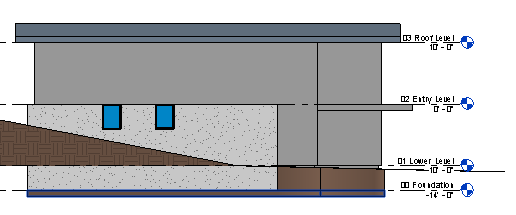
\includegraphics[width=\linewidth]{revitsouthernwindows.png}
			\caption{The Location of the Retaining Windows}
			\label{fig:revsouthwindows}
		\end{figure}
		
		\item Now go into the view: \menu{Side Bar > Project Browser > Floor Plans > 01 Lower Level}
		\clearpage
		\item If you do not see the windows in this view, go into these settings with the background selected: inside \menu{Side Bar > Properties > Extents > View Range > Primary Range > Cut Plane > Offset:} and set the number inside as \menu{6'0"}
		\item Now you can properly move the windows. Select the right window and move it until it is \menu{2'6"} from the right interior walls, and move the left window until it is \menu{9'6"} from the leftmost wall. Reference figure \ref{fig:revlowerwindowfinal}
		
		\begin{figure}
			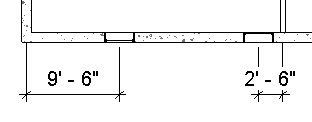
\includegraphics[width=\linewidth]{revitlowerwindowfinal.png}
			\caption{The Final Lower Level Windows}
			\emph{Your windows should look like this, annotations excluded}
			\label{fig:revlowerwindowfinal}
		\end{figure}
		
	\subsection{Entry Level Windows}
		\item You can use the same windows settings as in the previous section
		\item Go to view: \menu{Side Bar > Project Browser > Floor Plans > 02 Entry Level}
		
		\begin{marginfigure}
			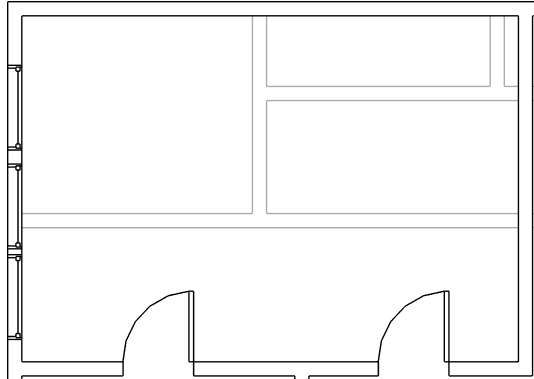
\includegraphics[width=\linewidth]{revitupperwindowinitial.png}
			\caption{The initial Entry Level Windows}
			\emph{Do not be worried if they are staggered, that will be dealt with}
			\label{fig:revupperwindowinit}
		\end{marginfigure}
		
		\item Place three windows on the leftmost wall of the \menu{Medium Size Bedroom} reference Figure \ref{fig:revupperwindowinit}
		\item Select the following tool: \menu{Annotate > Dimension > Aligned}
		\item Click on the items in this order: The topmost wall, the middle of the first window, the middle of the second window, the middle of the third window, and the room's bottommost wall. Reference Figure \ref{fig:revupperwindowaligned}
		
		\begin{marginfigure}
			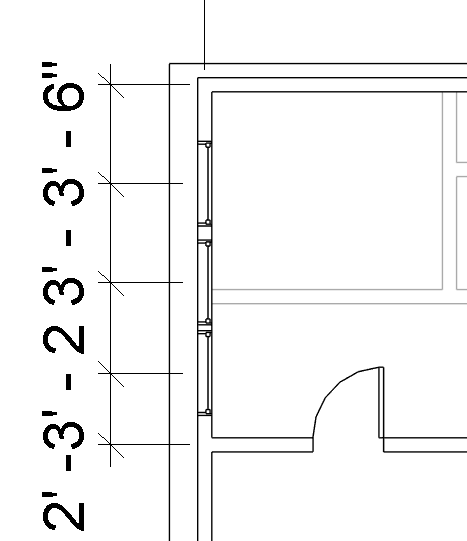
\includegraphics[width=\linewidth]{revitupperwindowaligned.png}
			\caption{The Upper Windows Aligned}
			\emph{Your windows should look like this with the alignment tool properly applied, they should not have changed yet.}
			\label{fig:revupperwindowaligned}
		\end{marginfigure}
		
		\item Click on the line which holds the alignment numbers, to the left of all the numbers should be a little symbol. It says \menu{EQ} with a line through it.
		\item Click on the little \menu{EQ}. All your windows should become equal in distance, and the numbers should change to EQ. Check figure \ref{fig:revupperwindowfinal}
		
		\begin{figure}
			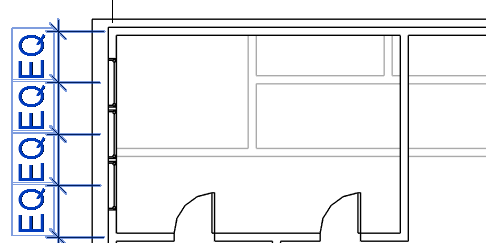
\includegraphics[width=\linewidth]{revitupperwindowfinal.png}
			\caption{Final Upper Window Arrangements}
			\emph{Your windows should look similar to this}
			\label{fig:revupperwindowfinal}
		\end{figure}
\end{enumerate}
		
\chapter{Chapter 7 - Creating a Curtain Wall, Connected Walls, and Entry Deck}
\label{ch:7}
In this section of the guide, you will be learning how to create new wall types, connecting walls to the roof, and creating an entry level deck.
\begin{enumerate}
\section{Creating a Curtain Wall}
	\item Open up to view: \menu{Side Bar > Project Browser > Floor Plans > 01 Lower Level}
	\item Using the \menu{Modify > Modify > Split Element} tool from when creating a hallway, split a point above the \menu{01 Lower Level} Exterior Door.
	\item Using the \keys{Ctrl + Click} combination your learned earlier, select the segment that you seperated from the wall, and the topmost \menu{Generic 6"} wall segment.
	
	\begin{marginfigure}
		\includegraphics[width=\linewidth]{revitcurtainwallinit.png}
		\caption[The Revit Curtain Wall Segments Selected]{These are the segments you should have split, and selected for the creation of the curtain walls.}
		\label{fig:revcurtwallinit}
	\end{marginfigure}
	
	\item With the segments selected, go into properties and give it the following:
	
	\newthought{}\begin{tabular}{c | c}
		Settings & \menu{Curtain Wall Storefront}\\
		\hline
		Location Line & Wall Centerline\\
		Base Constraint & \menu{01 Lower Level}\\
		Base Offset & \menu{0'0"}\\
		Top Constraint & Up to \menu{03 Roof Level}\\
		Top Offset & \menu{0'0"}\\
	\end{tabular}
	
	\item Refer to Figure \ref{fig:revcurtwallfinal}
	
	\begin{figure}
		\includegraphics[width=\linewidth]{revitcurtainwallfinal.PNG}
		\caption{The Final Curtain Wall Arrangement}
		\label{fig:revcurtwallfinal}
	\end{figure}
	\subsection{Creating a Unique Curtain Wall Type}
		\item Below the sections which allows you to change object types is the \menu{Edit Type} Button. If you click it, it gives you a more advanced version of the Object Options
		\item Click \menu{Side Bar > Properties > Edit Type}
		\item Inside, click the \menu{Duplicate...} Button. The name should be this: \menu{House 4x4}
		\item Change the following options to this:
		
		\newthought{}\begin{tabular}{c  c}
			\emph{Vertical Grid} \\
			\hline
			Spacing & \menu{4'0"}\\
			\hline
			\emph{Horizontal Grid} \\
			\hline
			Spacing & \menu{4'0"}
		\end{tabular}
		
		\item Click \menu{OK}
		\marginnote{If your walls are not visible in 3D view, click on the little Lightbulb at the bottom of the screen. Your screen should go purple and you will be able to see it. Right click the missing wall, and in the context menu, select \menu{Unhide in View > Element} and click the Lightbulb again}
		\item Go into the 3D view and admire your work.
		
		\begin{figure*}	
			\includegraphics[width=\linewidth]{revitcurtainwall3dviewfinal.png}
			\caption{The Finalized 3D Image of Curtain Walls}
			\emph{Yours should look rather similar to this}
			\label{fig:revcurtthreedfinal}
		\end{figure*}
\section{Attaching Walls to the Roof}
	\item If not given proper instruction, attaching walls to the roof may be challenging, but is actually one of the most simple exercises in Revit
	\item while in 3D view, \keys{Ctrl + Click} each exterior wall, excluding the Retaining walls.
	\item Reference Figure \ref{fig:revattachinit}
	\begin{figure}
		\includegraphics[width=\linewidth]{revitattachmentwallsinitial.png}
		\caption[All walls selected for attachment process]{Here all the walls are selected through \keys{Ctrl + Click}ing.}
		\emph{Notice! Use the gap between the walls and the roof to select the interior walls as well. If you click elsewhere and your selection disappears, right click, and a context menu will appears, select: \menu{Select Previous}. \keys{Shift + Click}ing also will remove a wall from your selection}	
	\end{figure}
	\item Then click on the tool: \menu{Modify | Walls > Modify Wall > Attach Top/Base}, and with all the walls still selected, click on the roof.
	\item Any alerts that show up, which may be on the bottom right of your screen, ignore, unless it says \menu{Delete Elements} in regards to the Curtain Wall Mullions, then click that option, if you have any concerns, reference a Instructor or Friend
	\item Now admire your attached walls and Curtain wall in the 3D view for a moment. Pat yourself on the back, you've made it further than most, but you're not done yet.
	\begin{figure*}
		\includegraphics[width=\linewidth]{revitattachfinal.png}
		\caption{The Recently Attached Walls}
		\emph{Note that the side door is missing in these past 3D visualizations, this is to keep the focus on the walls, and not the door.}
	\end{figure*}
\section{Creating the Entry Deck}
	\item Open the view: \menu{Side Bar > Project Browser > Floor Plans > 02 Entry Level}
	\item select the following tool: \menu{Architecture > Build > Floor}
	\item Create a new floor right outside the topmost wall. Pick a point close to where the top corner is of the current floor. When you choose that point, move up \menu{11'0"}
	\item Then, at the leftmost corner of the topmost wall, make a point and move up \menu{3'6"}
	\item Now connect the two points, reference figure \ref{fig:reventdeckinit}
	
	\begin{figure}
		\includegraphics[width=\linewidth]{revitsideentrydeckinit.png}
		\caption{A Correct Side Entry Deck}
		\emph{Yours should look very close to this. If not, then correct, or reference Instructor or friend}
		\label{fig:reventdeckinit}
	\end{figure}
	
\end{enumerate}
	
	
		


	

%----------------------------------------------------------------------------------------

\backmatter

%----------------------------------------------------------------------------------------
%	BIBLIOGRAPHY
%----------------------------------------------------------------------------------------

\bibliography{bibliography} % Use the bibliography.bib file for the bibliography
\bibliographystyle{plainnat} % Use the plainnat style of referencing

%----------------------------------------------------------------------------------------

\printindex % Print the index at the very end of the document

\end{document}